%%%% ijcai24.tex

\typeout{Formal Verification of  Parameterised Neural-symbolic Multi-agent Systems}

% These are the instructions for authors for IJCAI-23.

\documentclass{article}
\pdfpagewidth=8.5in
\pdfpageheight=11in

% The file ijcai23.sty is a copy from ijcai22.sty
% The file ijcai22.sty is NOT the same as previous years'
\usepackage{ijcai23}

\usepackage[T1]{fontenc}
\usepackage{amsmath,amssymb,mathtools}

% Use the postscript times font!
\usepackage{times}
\usepackage{soul}
\usepackage{url}
\usepackage[hidelinks]{hyperref}
\usepackage[utf8]{inputenc}
\usepackage[small]{caption}
\usepackage{graphicx}
\usepackage{amsmath}
\usepackage{amsthm}
\usepackage{booktabs}
\usepackage{algorithm}
\usepackage{algorithmic}
\usepackage{xspace}
\usepackage{paralist}
\usepackage[switch]{lineno}
\usepackage{tikz}
\usetikzlibrary{shapes}
\usepackage{marginnote}

% Comment out this line in the camera-ready submission
% \linenumbers

\urlstyle{same}

% the following package is optional:
%\usepackage{latexsym}

% See https://www.overleaf.com/learn/latex/theorems_and_proofs
% for a nice explanation of how to define new theorems, but keep
% in mind that the amsthm package is already included in this
% template and that you must *not* alter the styling.
\newtheorem{example}{Example}
\newtheorem{theorem}{Theorem}
\newtheorem{definition}{Definition}
\newtheorem{lemma}{Lemma}
\newtheorem{corollary}{Corollary}
\newtheorem{innercustomthm}{Theorem}
\newenvironment{customthm}[1]
  {\renewcommand\theinnercustomthm{#1}\innercustomthm}
  {\endinnercustomthm}
\newtheorem{innercustomlemma}{Lemma}
\newenvironment{customlemma}[1]
  {\renewcommand\theinnercustomlemma{#1}\innercustomlemma}
  {\endinnercustomlemma}


% Following comment is from ijcai97-submit.tex:
% The preparation of these files was supported by Schlumberger Palo Alto
% Research, AT\&T Bell Laboratories, and Morgan Kaufmann Publishers.
% Shirley Jowell, of Morgan Kaufmann Publishers, and Peter F.
% Patel-Schneider, of AT\&T Bell Laboratories collaborated on their
% preparation.

% These instructions can be modified and used in other conferences as long
% as credit to the authors and supporting agencies is retained, this notice
% is not changed, and further modification or reuse is not restricted.
% Neither Shirley Jowell nor Peter F. Patel-Schneider can be listed as
% contacts for providing assistance without their prior permission.

% To use for other conferences, change references to files and the
% conference appropriate and use other authors, contacts, publishers, and
% organizations.
% Also change the deadline and address for returning papers and the length and
% page charge instructions.
% Put where the files are available in the appropriate places.


% PDF Info Is REQUIRED.
% Please **do not** include Title and Author information
\pdfinfo{
/TemplateVersion (IJCAI.2023.0)
}

\title{Formal Verification of  Parameterised Neural-symbolic Multi-agent Systems}

% Single author syntax
\author{
    %Panagiotis Kouvaros
    %\affiliations
    %Imperial College London, London, UK
    %\emails
    %p.kouvaros@imperial.ac.uk
}

% Multiple author syntax (remove the single-author syntax above and the \iffalse ... \fi here)
\iffalse
\author{
First Author$^1$
\and
Second Author$^2$\and
Third Author$^{2,3}$\And
Fourth Author$^4$
\affiliations
$^1$First Affiliation\\
$^2$Second Affiliation\\
$^3$Third Affiliation\\
$^4$Fourth Affiliation
\emails
\{first, second\}@example.com,
third@other.example.com,
fourth@example.com
}
\fi

\newcommand{\tuple}[1]{\left ( #1  \right )}
\newcommand{\set}[1]{\left \{ #1  \right \}}
\newcommand{\ags}[0]{\it{Ag}}
\newcommand{\ag}[1]{{#1}}
\newcommand{\lstates}[1]{L_{#1}}
\newcommand{\lstate}[1]{l_{#1}}
\newcommand{\init}[1]{\iota_{#1}}
\newcommand{\plstate}[1]{l'_{#1}}
\newcommand{\pplstate}[1]{l''_{#1}}
\newcommand{\prvs}[1]{\it{Prv}_{#1}}
\newcommand{\pers}[1]{\it{Per}_{#1}}
\newcommand{\prv}[1]{\it{prv}_{#1}}
\newcommand{\per}[1]{\it{per}_{#1}}
\newcommand{\pprv}[1]{\it{prv}'_{#1}}
\newcommand{\pper}[1]{\it{per}'_{#1}}
\newcommand{\prot}[1]{\it{prot}_{#1}}
\newcommand{\obs}[1]{\it{obs}_{#1}}
\newcommand{\tr}[1]{\it{tr}_{#1}}
\newcommand{\sys}[1]{\mathcal{S}^{(#1)}}
\newcommand{\asys}[1]{\mathcal{S}_{ab}^{(#1)}}
\newcommand{\npis}{\mathcal{S}}
\newcommand{\agents}[1]{\it{Ag}^{(n)}}
\newcommand{\ls}[2]{\it{ls}_{#1}(#2)}
\newcommand{\lprv}[2]{\it{lprv}_{#1}(#2)}
\newcommand{\lper}[2]{\it{lper}_{#1}(#2)}
\newcommand{\globalacts}[1]{\it{ACT}^{(#1)}}
\newcommand{\aglobalacts}[1]{\it{ACT}^{(#1)}_{ab}}
\newcommand{\acts}[1]{\it{Act}_{#1}}
\newcommand{\act}[1]{\it{\alpha}_{#1}}
\newcommand{\la}[2]{\it{la}_{#1}({#2})}
\newcommand{\msys}[1]{\mathcal{M}_{\sys{#1}}}
\newcommand{\masys}[1]{\mathcal{M}_{\mathcal{S}_{ab}^{(#1)}}}
\newcommand{\globalstates}[1]{G^{(#1)}}
\newcommand{\globalinit}[1]{\iota^{({#1})}}
\newcommand{\globaltr}[1]{\it{tr}^{(#1)}}
\newcommand{\globalrel}[1]{T^{(#1)}}
\newcommand{\valuation}[1]{\ell^{(#1)}}
\newcommand{\aglobalstates}[1]{G^{(#1)}_{ab}}
\newcommand{\aglobaltr}[1]{\it{tr}^{(#1)}_{ab}}
\newcommand{\aglobalrel}[1]{T^{(#1)}_{ab}}
\newcommand{\aglobalinit}[1]{\iota^{({#1})}_{ab}}
\newcommand{\avaluation}[1]{\ell^{(#1)}_{ab}}
\newcommand{\tlabel}[1]{\ell_{#1}}
\newcommand{\prop}[0]{\it{AP}}
\newcommand{\ctl}[0]{\sf{CTL}}
\newcommand{\bctl}[0]{\sf{bCTL}}
\newcommand{\bictl}[0]{\sf{bICTL}}
\newcommand{\bictlspec}[0]{\forall_{v1_,\ldots,v_m} \varphi}
\newcommand{\atprop}{\it{AP}}
\newcommand{\atvar}{\it{VAR}}
% \newcommand{\paths}[1]{\Pi_{\sys n}(#1)}
% \newcommand{\apaths}[2]{\Pi_{\asys m}^{#2}(#1)}
\newcommand{\paths}[1]{\Pi(#1)}
\newcommand{\apaths}[2]{\Pi^{#2}(#1)}
\newcommand{\pathstates}[2]{\it{States}(\Pi^{#2}(#1))}

\newcommand{\pnis}{\mathcal S}
\newcommand{\apnis}{\overline{\mathcal S}}
\newcommand{\astates}{\overline{G}}
\newcommand{\aact}{\overline{ACT}}
\newcommand{\atr}{\overline{\it{tr}}}
\newcommand{\alabel}{\overline{{\ell}}}
\newcommand{\abstate}{q_{ab}}
\newcommand{\abstatep}{q_{ab}'}
\newcommand{\abaction}{\alpha_{ab}}
\newcommand{\abactionp}{\alpha_{ab}'}
\newcommand{\abpath}{\rho_{ab}}
\newcommand{\td}[1]{\it{td}(#1)}
\newcommand{\projection}[2]{#1_{\rightarrow #2}}





\begin{document}

\maketitle

\begin{abstract}

We study the problem of verifying multi-agent systems composed of arbitrarily
many neural-symbolic agents. We introduce a novel parameterised model, where the
parameter denotes the number of agents in the system, each homogeneously
constructed from an agent template equipped with a neural network-based
perception unit  and traditionally programmed action selection mechanism. We
define the verification and emergence identification problems for these models
against a bounded fragment of CTL. We put forward an abstraction methodology
that enables us to recast both problems to the problem of checking Neural
Interpreted Systems with a bounded number of agents. We present an
implementation and discuss experimental results obtained on a guarding scenario
of social dilemma games.



\end{abstract}

\section{Introduction}
Safety concerns emanating from the increasing development of Multi-agent Systems
(MAS) have been put under mathematical scrutiny over the past decade  in
automated methods that ascertain their correct behaviour. Verification methods
based on SAT and BDDs~\cite{KacprzakLomuscioPenczek04b,RaimondiLomuscio05c} have
resulted in push-button engines such as Verics, MCK and
MCMAS~\cite{GammieMeyden04a,Kacprzak+07a,LomuscioQuRaimondi15}.  In conjunction
with increasingly sophisticated state-space reduction methods, such as predicate
absrtaction~\cite{lomuscio2015verifying} and partial order
reductions~\cite{jamroga2020towards}, the verifiers have been able to scale to
the analysis of systems with very large state spaces.


While the different methods target the provision of effective solutions to
different types of analyses, e.g., fast search for
counterexamples~\cite{penczek2003verifying} as opposed to fast correctness
proofs~\cite{ball2006abstraction} and for different classes of MAS, e.g., MAS
defined over infinite-state as opposed to finite-state
variables~\cite{lomuscio2015verifying}, all methods make two fundamental
assumptions. The first is that the MAS under analysis is composed of a known
number of agents specified at design time. The second is that the agents
composing the MAS are specified using traditional programming languages.  The
approaches cannot in principle therefore be used to verify important classes of
MAS, where either the systems have arbitrarily many participants or the agents 
are endowed with machine learning components. The former class of systems
includes open systems, where agent can join and leave the system at runtime, and
applications designed irrespective of the number of participants such as robot
swarms and scenarios in the Internet of Things. The latter class comprises
forthcoming neural-symbolic applications such as autonomous vehicles.

More recent methods have addressed the verification of systems with an unbounded
number constituents against agent-based
specifications~\cite{KouvarosLomuscio16a,KouvarosLomuscio15b,KouvarosLomuscio16c}.
While the different methods focus on different communication primitives for the
agents, they all rely on either cutoffs or zero-one abstractions whereby
the unbounded verification problem is reduced to verifying a small
number of concrete systems or abstractions thereof.  

In a different line of work verification methods for MAS comprising agents with 
neural components were put forward~\cite{Akintunde+20b,Akintunde+22}. To deal
with the real-valued operational domain of the networks the methods recast
verification queries for bounded properties into
Mixed-Integer-Linear-Programming.

While these lines of work independently tackle unbounded and neural-symbolic
MAS, none of the underlying methods can be used for analysis of systems that are
both unbounded and neural-symbolic.  In this paper we overcome this limitation.
We specifically introduce Parameterised Neural Intepreted Systems (PNIS), a
formal model based on neural interpreted systems for modelling unbounded
neural-symbolic MAS.  We develop an abstraction methodology for PNIS whereby we
derive sound and complete procedures for the verification and emergence
identification problems with respect to  bounded universal and existential CTL
formulae. 

% \end{itemize}

The rest of the paper is organised as follows. After discussing related work
below, we present PNIS in Section~\ref{sec:pnis}, followed by the development of
their verification and emergence identification procedures in
Section~\ref{sec:verification}, which we evaluate in Section~\ref{sev:eval}  on a social
dilemma scenario. We conclude in Section~\ref{sec:conclusions}.


{\bf Related Work.}  The contribution is related to the two lines of work
discussed above, namely parameterised verification and verification for
neural-symbolic MAS. Previous models in parameterised verification do not
include neural components, which require the formulation of novel abstractions.
The neural components here considered additionally restrict the analysis to
bounded temporal formulae, thereby however enabling the derivation of sound and
complete verification methods for both universal and existential properties, as
opposed for only universal properties that typically concerns previous work.
Verification methods for MAS with neural components were previously put forward.
These however take as input MAS with a known number of agents. The main
theoretical findings of this  the paper is that verification in the unbounded
case can be reduced to the verification of a small number of bounded models from
the cited work.

% hese include
% SAT-based and BDD-based verification methods (Kacprzak,
% Lomuscio, and Penczek 2004; Raimondi and Lomuscio
% 2005). Current model checkers, such as Verics, MCK and
% MCMAS (Kacprzak et al. 2008; Gammie and van der Mey-
% den 2004; Lomuscio, Qu, and Raimondi 2015), can effi-
% ciently verify large state-spaces.

% Recent advances in  Artificial Intelligence (AI)  enabled the automation of
% challenging tasks, such as computer vision, that have been traditionally
% difficult to tackle for decades. This accelerated the incorporation of  AI
% components in  diverse applications, including ones situated within domains, such as
% healthcare and transportation, where the impact to society can be significant.
% While however AI has the potential of revolutionising society,  its inherent
% fragility and opacity   hinders its adoption in safety-critical applications.
% The associated risks are compounded in an increasingly inter-connected
%Still, even though there is an increasing consensus in AI being beneficial for
%society,  its inherent fragility and opacity hinders its adoption in
%safety-critical applications. The associated risks are compounded in an
%increasingly inter-connected
% socio-techno-economic
% world, where systems of
% multiple interacting intelligent agents, or multi-agent systems (MAS),
% constitute a paradigm shift from object-oriented to interaction-oriented design
% standards. 

% In response to these concerns the area of formal verification of AI has grown
% rapidly over the past few years to provide methods to automatically verify that
% AI systems robustly behave as intended.
% One of the key techniques that has emerged in the area is that of {\em model
% checking}~\cite{Clarke+99a}. Model checking provides automated solutions to 
% the problem of establishing whether a model $M_S$ representing a system $S$ satisfies a
% logical formula $\phi_P$ encoding a specification $P$. In the case of MAS,
% the formula $\varphi$ does not simply express temporal properties of systems, as
% in reactive systems, but it may also be accounting for high-level attitudes of
% agency, such as knowledge and strategies, which can be described in
% temporal-epistemic logic~\cite{Fagin+95b} and alternating-time
% logic~\cite{Alur+98a}.

% Whilst methods such as binary binary decision diagrams~\cite{GammieMeyden04a}
% and bounded model checking~\cite{PenczekLomuscio03b}   enabled the  model
% checking  of systems of large state spaces, a main drawback of the approach
% remains the state-space explosion problem, whereby the state-space grows
% exponentially in the number of variables encoding the agents.

%growth of the state space in the number of
%variables encoding the agents.

% Notwithstanding that in practice this limits model checking to the verification
% of systems with only few constituents, the analysis of  systems with arbitrarily many
% participants, such as robot swarms  and  applications in the Internet of Things, 
% raises a principal barrier to its application.  Indeed, 
% verifying systems of this kind, henceforth {\em unbounded multi-agent systems}
% (UMAS), requires checking whether any system for any number of agents satisfies
% the specification in question. This  renders model checking intractable when 
% enumerating and analysing all individual systems. 


% The formal verification problem is concerned withV
% $S$ satisfies a safety property $P$. {\em Model checking}, a key method for the
% formal verification of reactive systems, has also been used in the past fifteen
% years to provide automated solutions to this problem~\cite{Clarke+99a}. In
% model checking, the system is represented as a model $M_S$, the specification
% is encoded as formula $\varphi$ and it is then checked whether $M_S$ satisfies
% $\varphi$. 

% In these cases, one could encode a system with a given number of agents and
% verify that a specification holds. However, additional agents may possibly
% interfere with the system in unpredictable ways resulting in the specifications
% being violated. Therefore, to fully verify the system, the process would have to
% be repeated for any possible number of components

% Another key limitation of model checking is the requirement that the systems are
% given in traditional, agent-based programming languages, thereby not accounting for  
%  agents endowed with neural network components.
% Systems of this kind, henceforth {\em neuro-symbolic multi-agent systems}
% (NMAS), constitute important forthcoming applications, such as autonomous
% vehicles, where the neural components are responsible for automating complex tasks such
% as perception and control. 

% Even though neural networks exhibit remarkable performance on these tasks,
% their fragility to adversarial attacks~\cite{Szegedy+14} and
% their lack of interpretability~\cite{VelizKim17} raise additional concerns
% regarding the overall system safety, thereby strengthening the need for the
% principled analysis of NMAS before deployment.

% This paper gives an overview of the methods that we developed within the
% Verification of Autonomous Systems Research
% Group, Imperial College London, 
% %~\footnote{\url{https://vas.doc.ic.ac.uk}} 
% towards the formal verification
% of UMAS and NMAS.  Our pioneering work in the verification of UMAS, discussed in
% Section~2, overcomes the model checking barrier with the development of methods
% that enable the derivation of the number of agents that is sufficient to
% consider when evaluating a specification. Our studies in the analysis of NMAS,
% outlined in Section~3, include efficient methods for the verification of neural
% networks and mixed-integer linear programming (MILP) formulations for checking
% system-level specifications.  The paper concludes in Section~4 with directions
% for future work.


\section{Parameterised Neural-symbolic Interpreted Systems}
\label{sec:pnis}
Interpreted systems are a standard semantics for describing multi-agent systems
[Fagin et al., 1995b]. They provide a natural setup to interpret specifications
in a variety of languages including temporal-epistemic logic and alternating
temporal logic [Fagin et al., 1995a; Lomuscio and Raimondi, 2006].
Parameterised interpreted systems is a parametric extension of interpreted
systems put forward to reason about unbounded multi-agent
systems~\cite{KouvarosLomuscio15b}. The parameter in a system of this kind
denotes the number of agents composing the system, each homogeneously
constructed from an agent template. We here extend parameterised interpreted
systems to Parameterised Neural-symbolic Interpreted Systems (PNIS), where the
template for the agents is not purely symbolic but it comprises a perception
mechanism that is implemented via neural networks and which is coupled with a
symbolic action mechanism. This neural-symbolic treatment of the agents follows
the Neural Interpreted Systems (NIS) model from~\cite{Akintunde+20b}.
Differently from NPIS however, NIS are limited to standard non-parametric
systems with a pre-defined number of agents.

A PNIS consists of the descriptions of an agent template, from which an
unbounded number of concrete agents may be constructed, and an environment in
which the agents operate. The agent template is defined by the following. 

\begin{definition}[Agent template.]
An {\em agent template} is a tuple $\ag t = \tuple{\lstates t, \init t, \obs t,
\acts t, \prot t, \tr t }$, where:
\begin{itemize}
  \item $\lstates t = \prvs t \times \pers t$ is a nonempty (possibly infinite)
  set of local states.  Each local state  is a pair $\tuple{\prv t, \per t}$ of
  a private state $\prv t \in \prvs t \subseteq \mathbb R^{m_{prv}}$ and a
  percept $\per t \in \pers t \subseteq \mathbb R^{m_{per}}$ that encodes the
  perception a agent has about the environment.  

  \item $\init t \in \lstates t$ is the unique initial template state.
  
  \item $\obs t : \lstates t \times \lstates e \rightarrow \pers t$ is an
  observation function that maps pairs of template local states $\lstates t
  \subseteq \mathbb{R}^{m_{prv} + m_{per}}$ and environment states $\lstates e
  \subseteq \mathbb{R}^{m_e}$ (defined below) to percepts $\pers t \subseteq
  \mathbb{R}^{m_{per}}$. The observation function is implemented via a PWL FFNN $f :
  \mathbb{R}^{m_{prv} + m_{per} + m_e} \rightarrow \mathbb{R}^{m_{per}}$.

  \item $\acts t$ is a nonempty and finite set of actions.
  
  \item $\prot t : \lstates t \rightarrow 2^{\acts t} \setminus \set{\emptyset}$
  is a local protocol function that selects which actions may be performed at a
  given local state.%%\nb{E: shouldn't the protocol take as input $\pers{t}$?}

  \item $\tr t: \lstates t \times \acts t \times 2^{\acts t} \times \acts e 
  \rightarrow \prvs t$ is a local transition function  that determines the next
  private state for a concrete agent given its current local state, its action, 
  the set of actions performed by all the agents  and the action of the
  environment.
  
\end{itemize}  
\end{definition}

% \begin{example}
%   \label{ex:agent-template}
%   We consider the example of a guarding game, an instance of sequential social
%   dilemma games \cite{LeiboZLMG17}.\nb{E: check if this is really an SSD} In this game there is a colony of
%   agents. The colony needs to be guarded by exactly one guard. Guarding duty
%   costs the guard some health, $G_p$, while those who are resting improve their
%   health by $R_r$, where the health is limited by a maximum value $M_h$. If no
%   one is guarding the colony, then all the agents in the colony lose some
%   health, $U_p$. When an agent does not have any health left, it
%   \emph{expires}.

%   We formalise the agent template
%   $\ag t = \tuple{\lstates{t}, \init{t}, \obs{t}, \acts{t}, \prot{t}, \tr{t} }$
%   in this game as follows.

 
%   \begin{itemize}[$\bullet$]
%   \item
%     $\lstates{t} = \{(h,\per{}) \mid h \in \{0,\dots,M_h\}, \ \per{} \in \{G_s,
%     R_s, E_s\}$, where $h$ is an integer between 0 and $M_h$, denoting the
%     health of the agent, while percepts $G_s$, $R_s$ and $E_s$ indicate what
%     actions are available to the agent depending on its health.
%     % stand for \emph{G}uarding, \emph{R}esting and \emph{E}xpired
%     % \emph{s}tates, respectively.

%   \item $\init{t} = (G_p + 1, G_s)$, i.e., at the start each agent has enough
%     of health to be able to guard at least once without expiring.
    
%   \item $\acts{t} = \{G_a, R_a, E_a\}$, where $G_a$, $R_a$ and $E_a$ stand for
%     \emph{G}uarding, \emph{R}esting and \emph{E}xpired \emph{a}ctions,
%     respectively.
  

%   \item Normally, we assume that the observation function is given as a
%     FFNN. But for the sake of illustration, we define here the observation
%     function of a perfectly altruistic agent:

%     $\obs{t}((h,\per{}), \ \lstate{e}) = \left\{
%       \begin{array}{rl}
%         G_s, & \text{ if } h > G_p\\ 
%         R_s, & \text{ if } 0 < h \leq G_p\\ 
%         E_s, & \text{ if } h \leq 0\\
%       \end{array} \right.$
    
%     Intuitively, if health is good enough, then the agent is in a position to
%     guard, if health is still positive, the agent can only rest, otherwise the
%     agent is ``expired''. In this example, the environment state is ignored by
%     the observation function.
    
%   \item $\prot{t}(h,\per{}) = \left\{
%       \begin{array}{rl}
%         \{G_a, R_a\}, & \text{ if } \per{} = G_s\\ 
%         \{R_a\}, & \text{ if } \per{} = R_s\\ 
%         \{E_a\}, & \text{ if } \per{} = E_s\\
%       \end{array} \right.$

%     If the percept is $G_s$, then the agent can both guard and rest. If the
%     percept is $R_s$ or $E_s$, the only available actions are resting and the
%     dummy action $E_a$, respectively.
    
%   \item The local transition function ensures that at most one agent guards at
%     any moment. Formally, for $S \in \{G_s,R_s\}$:

%     %% no restriction on everybody guarding
%     %% suitable for existential properties only
%     $\begin{array}{@{}l@{\quad}l}\small
%        \tr{t}((h,S), G_a, A) = \max(h - G_p,0) &\\% \text{ and } h > G_p\\
%        % \tr{t}((h,S), G_a, A) = 0     &\text{ if }G_a\notin A \text{ and } h \leq G_p\\[2mm]
%        \tr{t}((h,S), R_a, A) = \min(h + R_r, M_h) &\text{ if }G_a\in A\\
%        \tr{t}((h,S), R_a, A) = \max(h - U_p,0) &\text{ if }G_a\notin A\\% \text{ and } h > U_p\\
%        % \tr{t}((h,S), R_a, A) = 0     &\text{ if }G_a\notin A \text{ and } h \leq U_p\\[2mm]
       
%        \tr{t}((h,E_s), E_a, A) = h\\
%      \end{array}$

%      %% restrictions on everybody guarding or resting.
%      %% suitable for universal properties as well
%      $\begin{array}{@{}l@{\quad}l}\small
%         \tr{t}((h,S), G_a, A) = \max(h - G_p,0) &\text{ if }R_a \text{ or }S_a\text{ in } A\\% \text{ and } h > G_p\\
%         \tr{t}((h,S), G_a, A) = -1 &\text{ if }\{G_a\} = A\\% \text{ and } h > G_p\\
%         % \tr{t}((h,S), G_a, A) = 0     &\text{ if }G_a\notin A \text{ and } h \leq G_p\\[2mm]
%        \tr{t}((h,S), R_a, A) = \min(h + R_r, M_h) &\text{ if }G_a\in A\\
%        \tr{t}((h,S), R_a, A) = \max(h - U_p,0) &\text{ if }G_a\notin A\\% \text{ and } h > U_p\\
%        % \tr{t}((h,S), R_a, A) = 0     &\text{ if }G_a\notin A \text{ and } h \leq U_p\\[2mm]
       
%        \tr{t}((h,E_s), E_a, A) = h\\
%      \end{array}$
% \end{itemize}

% \end{example}

\begin{example}
      %% no restriction on everybody guarding
    %% suitable for existential properties only

  \label{ex:agent-template}

  Version 1, Everybody can guard and rest
  
  We consider the example of a guarding game, an instance of sequential social
  dilemma games \cite{LeiboZLMG17}.\nb{E: check if this is really an SSD} In
  this game there is a colony of agents. The colony needs to be
  guarded. Guarding duty costs the guard some health~$G_p$, while those who
  are resting improve their health by $R_r$, where the health is limited by a
  maximum value $M_h$. If no one is guarding the colony, then all the agents in
  the colony lose some health, $U_p$. When an agent does not have any health
  left, it \emph{expires}.

  We formalise the agent template
  $\ag t = \tuple{\lstates{t}, \init{t}, \obs{t}, \acts{t}, \prot{t}, \tr{t} }$
  in this game as follows.

 
  \begin{itemize}[$\bullet$]
  \item
    $\lstates{t} = \{(h,\per{}) \mid h \in \{0,\dots,M_h\}, \ \per{} \in \{G_s,
    R_s, E_s\}$, where $h$ is an integer between 0 and $M_h$, denoting the
    health of the agent, while percepts $G_s$, $R_s$ and $E_s$ indicate what
    actions are available to the agent depending on its health.
    % stand for \emph{G}uarding, \emph{R}esting and \emph{E}xpired
    % \emph{s}tates, respectively.

  \item $\init{t} = (G_p + 1, G_s)$, i.e., at the start each agent has enough
    of health to be able to guard at least once without expiring.
    
  \item $\acts{t} = \{G_a, R_a, E_a\}$, where $G_a$, $R_a$ and $E_a$ stand for
    \emph{G}uarding, \emph{R}esting and \emph{E}xpired \emph{a}ctions,
    respectively.
  

  \item Normally, we assume that the observation function is given as a
    FFNN. But for the sake of illustration, we define here the observation
    function of a perfectly altruistic agent:

    $\obs{t}((h,\per{}), \ \lstate{e}) = \left\{
      \begin{array}{rl}
        G_s, & \text{ if } h > G_p\\ 
        R_s, & \text{ if } 0 < h \leq G_p\\ 
        E_s, & \text{ if } h \leq 0\\
      \end{array} \right.$
    
    Intuitively, if health is good enough, then the agent is in a position to
    guard, if health is still positive, the agent can only rest, otherwise the
    agent is ``expired''. In this example, the environment state is ignored by
    the observation function.
    
  \item $\prot{t}(h,\per{}) = \left\{
      \begin{array}{rl}
        \{G_a, R_a\}, & \text{ if } \per{} = G_s\\ 
        \{R_a\}, & \text{ if } \per{} = R_s\\ 
        \{E_a\}, & \text{ if } \per{} = E_s\\
      \end{array} \right.$

    If the percept is $G_s$, then the agent can both guard and rest. If the
    percept is $R_s$ or $E_s$, the only available actions are resting and the
    dummy action $E_a$, respectively.
    
  \item The local transition function ensures that at most one agent guards at
    any moment. Formally, for $S \in \{G_s,R_s\}$:

    $\begin{array}{@{}l@{\quad}l}\small
       \tr{t}((h,S), G_a, A) = \max(h - G_p,0) &\\% \text{ and } h > G_p\\
       % \tr{t}((h,S), G_a, A) = 0     &\text{ if }G_a\notin A \text{ and } h \leq G_p\\[2mm]
       \tr{t}((h,S), R_a, A) = \min(h + R_r, M_h) &\text{ if }G_a\in A\\
       \tr{t}((h,S), R_a, A) = \max(h - U_p,0) &\text{ if }G_a\notin A\\% \text{ and } h > U_p\\
       % \tr{t}((h,S), R_a, A) = 0     &\text{ if }G_a\notin A \text{ and } h \leq U_p\\[2mm]
       
       \tr{t}((h,E_s), E_a, A) = h\\
     \end{array}$

\end{itemize}

\end{example}

% \begin{example}
%      %% restrictions on everybody guarding or resting.
%      %% suitable for universal properties as well
%   \label{ex:agent-template2}
%   Version 2
  
%   We consider the example of a guarding game, an instance of sequential social
%   dilemma games \cite{LeiboZLMG17}.\nb{E: check if this is really an SSD} In this game there is a colony of
%   agents. The colony needs to be guarded by exactly one guard. Guarding duty
%   costs the guard some health, $G_p$, while those who are resting improve their
%   health by $R_r$, where the health is limited by a maximum value $M_h$. If no
%   one is guarding the colony, then all the agents in the colony lose some
%   health, $U_p$. When an agent does not have any health left, it
%   \emph{expires}.

%   We formalise the agent template
%   $\ag t = \tuple{\lstates{t}, \init{t}, \obs{t}, \acts{t}, \prot{t}, \tr{t} }$
%   in this game as follows.

 
%   \begin{itemize}[$\bullet$]
%   \item
%     $\lstates{t} = \{(h,\per{}) \mid h \in \{0,\dots,M_h\}, \ \per{} \in \{G_s,
%     R_s, E_s\}$, where $h$ is an integer between 0 and $M_h$, denoting the
%     health of the agent, while percepts $G_s$, $R_s$ and $E_s$ indicate what
%     actions are available to the agent depending on its health.
%     % stand for \emph{G}uarding, \emph{R}esting and \emph{E}xpired
%     % \emph{s}tates, respectively.

%   \item $\init{t} = (G_p + 1, G_s)$, i.e., at the start each agent has enough
%     of health to be able to guard at least once without expiring.
    
%   \item $\acts{t} = \{G_a, R_a, E_a\}$, where $G_a$, $R_a$ and $E_a$ stand for
%     \emph{G}uarding, \emph{R}esting and \emph{E}xpired \emph{a}ctions,
%     respectively.
  

%   \item Normally, we assume that the observation function is given as a
%     FFNN. But for the sake of illustration, we define here the observation
%     function of a perfectly altruistic agent:

%     $\obs{t}((h,\per{}), \ \lstate{e}) = \left\{
%       \begin{array}{rl}
%         G_s, & \text{ if } h > G_p\\ 
%         R_s, & \text{ if } 0 < h \leq G_p\\ 
%         E_s, & \text{ if } h \leq 0\\
%       \end{array} \right.$
    
%     Intuitively, if health is good enough, then the agent is in a position to
%     guard, if health is still positive, the agent can only rest, otherwise the
%     agent is ``expired''. In this example, the environment state is ignored by
%     the observation function.
    
%   \item $\prot{t}(h,\per{}) = \left\{
%       \begin{array}{rl}
%         \{G_a, R_a\}, & \text{ if } \per{} = G_s\\ 
%         \{R_a\}, & \text{ if } \per{} = R_s\\ 
%         \{E_a\}, & \text{ if } \per{} = E_s\\
%       \end{array} \right.$

%     If the percept is $G_s$, then the agent can both guard and rest. If the
%     percept is $R_s$ or $E_s$, the only available actions are resting and the
%     dummy action $E_a$, respectively.
    
%   \item The local transition function ensures that at most one agent guards at
%     any moment. Formally, for $S \in \{G_s,R_s\}$:


%      $\begin{array}{@{}l@{\quad}l}\small
%         \tr{t}((h,S), G_a, A) = \max(h - G_p,0) &\text{ if }R_a \text{ or }S_a\text{ in } A\\% \text{ and } h > G_p\\
%         \tr{t}((h,S), G_a, A) = -1 &\text{ if }\{G_a\} = A\\% \text{ and } h > G_p\\
%         % \tr{t}((h,S), G_a, A) = 0     &\text{ if }G_a\notin A \text{ and } h \leq G_p\\[2mm]
%        \tr{t}((h,S), R_a, A) = \min(h + R_r, M_h) &\text{ if }G_a\in A\\
%        \tr{t}((h,S), R_a, A) = \max(h - U_p,0) &\text{ if }G_a\notin A\\% \text{ and } h > U_p\\
%        % \tr{t}((h,S), R_a, A) = 0     &\text{ if }G_a\notin A \text{ and } h \leq U_p\\[2mm]
       
%        \tr{t}((h,E_s), E_a, A) = h\\
%      \end{array}$
% \end{itemize}

% \end{example}

% \begin{example}\em
%   \label{ex:penguin-agent-template}
%   We consider the example of a penguin colony, an instance of sequential social
%   dilemma games \cite{LeiboZLMG17}.\nb{E: check if this is really an SSD} In
%   this scenario, there is a colony of penguins living in a very cold
%   environment. For a penguin to survive, it needs to maintain its body
%   temperature within a certain interval: if the body temperature drops too low
%   and raises too high, the penguin dies (here we assume a simplification of the
%   real-life dynamics).

%   We assume that penguins live on a
%   hexagonal grid. Given the cell where a penguin is located, there are 6
%   neighbouring cells (thus, there can be at most 6 neighbours). 

%   \def\r{3}%4}
%   \def\d{6}%8}
%   \def\w{5.2}%6.93} % r * sqrt(3)
%   \newcommand{\coord}[3]{\textcolor{purple}{#1},\! \textcolor{teal}{#2},\! \textcolor{violet}{#3}}
%   \begin{center}
%     \begin{tikzpicture}[%
%       hexagon/.style={draw=gray,  regular polygon, regular polygon
%         sides=6, minimum height=#1, rotate=30},
%       hexagon/.default={6mm}]     
%       \foreach \x in {1,2,...,4} { %
%         \foreach \y in {1,2} { %
%           \node[hexagon] at (\x*\w mm,\y*3*\r mm) {};
          
%           \node[hexagon] at (0.5*\w mm + \x*\w mm,1.5*\r mm+\y*3*\r mm) {};
%           % 
%         }}

%       \begin{scope}[xshift=5cm, yshift=1.5cm]
%         \node[hexagon=8mm] {};

%         % \node[scale=0.5] {\coord{0}{0}{0}};

%         \foreach \a/\n/\q/\r/\s in {%
%           60 /1/ 1/-1/ 0,%
%           0  /2/ 1/ 0/-1,%
%           300/3/ 0/ 1/-1,%
%           240/4/-1/ 1/ 0, %
%           180/5/-1/ 0/ 1, %
%           120/6/ 0/-1/ 1%
%         } {%
%           \node[hexagon=8mm] at (\a:6.93 mm) {};
          
%           \node[scale=0.5] at (\a:7.7 mm) {\n};%\coord{\q}{\r}{\s}};
          
%           \draw[-latex] (\a:0.25cm) -- (\a:0.55cm);%
%         }
%       \end{scope}
%     \end{tikzpicture}
%   \end{center}

%   We assume cube coordinates \cite{Patel21} for encoding the locations on the
%   hexagonal grid. Such coordinate system allows for standard vector operations,
%   for instance, given a current location $c$ and a vector of movement $a$, we
%   can compute the resulting location as $c+a$ (although in the example we
%   abstract away the exact coordinates). Assume that
%   $\mathit{Loc} \subseteq \mathbb{Z}^3$ is the arena, a set of connected
%   locations each identified by a 3d coordinate.

%   Penguins radiate heat in each of the 6 directions where there are no
%   neighbours, while for each direction where there is a neighbour the penguin
%   gains/preserves some heat. Let $r$ be the amount of heat radiated in one
%   direction. We assume the following update function for the temperature of a
%   penguin with $n$ neighbours:
%   $\mathit{upd}(t,n) = t - (6-n)\cdot r + n\cdot\frac{r}{2}$.
%   %
%   We number the directions 1 to 6 as in the figure
%   above, and denote the corresponding vectors as $v_1,\dots,v_6$. Let
%   $D = \{1,\dots,6\}$ be the set of all 6 directions.


%   We formalise the agent template
%   $\ag t = \tuple{\lstates{t}, \init{t}, \obs{t}, \acts{t}, \prot{t}, \tr{t} }$
%   in this scenario as follows.

 
%   \begin{itemize}[$\bullet$]
%   \item
%     $\lstates{t} = \{(c,t,f) \mid c \in \mathit{Loc}, \ t \in \mathbb{Z}, \ f
%     \in 2^D$, where $c$ is a 3d coordinate, $t$ an integer between 0 and $M_t$,
%     denoting the temperature of the penguin, while $f$ is a percept that is a
%     set of \emph{free} directions, indicating what neighbouring cells are
%     empty.

%   \item $\init{t} = ((0,0,0),t_0, D)$, the penguin has no neighbours.
    
%   \item $\acts{t} = \mathit{Loc}$, the actions encode the new location of a
%     penguin. % $\cup \{s\}$, where $m_l$
%     % is the action for moving to the location $l$ and $s$ for not moving.

%   \item $\obs{t}((c,t,f), \ \lstate{e}) = freedir(c,\lstate{e})$ (we will
%     define the environment state the function below)..
    
    
%   \item $\prot{t}(c,t,f) = \left\{
%       \begin{array}{rl}
%         \{c + v_i \mid i \in f\}, & \text{ if } f \neq \emptyset\\ 
%         \{c\}, & \text{ if } f = \emptyset\\ 
%       \end{array} \right.$

    
%   \item $\tr{t}((c,t, f), a, A, \act{e}) = (a, \mathit{upd}(t,n))$, where
%     $n = 6 - |f|$, i.e., the transition function updates the location and the
%     temperature of the penguin.
%   \end{itemize}

% \end{example}



An environment template has a similar description to an agent template but does
not include a perception mechanism.

\begin{definition}[Agent environment.]
An {\em agent environment} is a tuple $\ag e = \tuple{\lstates e, \acts e, \prot
e, \tr e }$, where $\lstates e  \subseteq \mathbb R^{m_e}$ is a nonempty
(possibly) infinite set of local states, $\acts e$ is a nonempty and finite set
of actions,  $\prot e : 2^{\acts e} \setminus \set{\emptyset}$ is a local
protocol function, and $\tr e : \lstates e \times \acts e \times 2^{\acts t} 
\rightarrow \lstates e$ is a local transition function.
\end{definition}

\begin{example}
  For the penguin scenario, the environment $e$ is defined as
  $\tuple{\lstates{e}, \acts{e}, \prot{e}, \tr{e}}$, where
  \begin{itemize}[$\bullet$]
  \item $\lstates{e} = \{(c,b) \mid c \in \mathit{Loc}, b\in\{0,1\}\}$. Thus
    every state is a map indicating whether there is at least one or no
    penguins at a location.
  \item $\acts{e} = \{0\}$
  \item $\prot{e} = ..$
  \item
    $\tr{e}(\mathit{map}, \act{e}, A) = A \times \{1\} \ \cup \
    (\mathit{Loc}\setminus A) \times \{0\}$ the transition function computes
    the new map, given the set of penguin actions.
  \end{itemize}
\end{example}

Agent and environment templates define the main formal structure we will be
using in this paper.

\begin{definition}[Parameterised Neural Interpreted System]
  A {\em Parameterised Neural Interpreted System} (PNIS) is a tuple $\mathcal S
  = \tuple{\ag t, \ag e, \ell}$, where $\tlabel{} : \atprop \rightarrow
  2^{\lstates t}$ is a labelling function on the agent  template states for a set
  $\atprop$ of atomic propositions.
\end{definition}

\begin{example}
  \label{ex:pnis}
  Consider the agent template in Example~\ref{ex:agent-template}.

  Assume that $e$ is.. %any environment (it is irrelevant for this example).
  
  Suppose $\atprop = \{\mathsf{a}, \mathsf{d}\}$, where $\mathsf{a}$ stands for
  alive and $\mathsf{d}$ for dead. Then we can define the labelling function
  $\ell$ as $\ell(\mathsf{a}) = \{(h,S) \mid h > 0 \text{ and }S \neq E_s\}$
  and $\ell(\mathsf{d}) = \lstates{t} \setminus \ell(\mathsf{a})$.
\end{example}

A PNIS $\mathcal S$ gives a parametric description of an unbounded collection
of {\em concrete} NIS. In particular, for any value $n \geq 1$ of the parameter
the concrete system $\sys n$ composes~$n$ copies $\ag 1, \ldots, \ag n$ of the
agent template with the environment $\ag e$. We write $\agents n$ for the set
$\agents n = \set{\ag 1, \ldots, \ag n}$ of concrete agents instantiated from
$\ag t$.
%
A \emph{global state} $q = \tuple{\lstate 1, \ldots, \lstate n, \lstate e}$ in
$\sys n$ is a tuple of local states for all the agents and the environment in
$\sys n$; it describes the system at a particular instant of time.  For a
global state $g$, we write $\lprv{a}{q}$, $\lper{a}{q}$ and $\ls{a}{q}$ to
denote the \emph{private part} $\prv a$ and the \emph{perception part} $\per a$
of the local state $\ls{a}{g} = \tuple{\prv a, \per a}$ of agent $\ag a$ in
$g$.  The set $\globalstates{n}=\lstates{1}\times\dots\times\lstates{n}\times L_e$
of all possible global states is the Cartesian product of the agents' sets of
local states.
% 
A \emph{joint action} $\alpha = \tuple{\alpha_1, \ldots, \alpha_n, \alpha_e}$
in $\sys n$ is a tuple of local actions for all the agents and the environment.
For a joint action $\alpha$, we write $\la{a}{\alpha}$ to denote the
\emph{local action} of agent $\ag a$ in~$\alpha$.  The set
$\globalacts{n} = \acts{1}\times\dots\times\acts{n}\times\acts{e}$ of all
possible joint actions is the Cartesian product of the agents' sets of local
actions.  A concrete system's global states evolve over time in compliance with
the following global transition relation.

% , i.e., for each agent $a \in \set{1,\ldots,n}$ we have that $a =
% \tuple{\lstates a, \init a, \obs a, \acts a, \prot a, \tr a} = \ag t$, 

\begin{definition}[Concrete Neural Interpreted System]
  \label{def:concreteystem}
Given an NPIS $\mathcal S = \tuple{\ag t, \ag e, \ell_t}$ and $n \geq 1$, a
\emph{concrete neural interpreted system} is a tuple $\sys n = \tuple{ \set{\ag 1,
\ldots, \ag n, \ag e}, \globalinit n, \valuation n}$, where $\globalinit n =
\tuple{\init 1, \ldots, \init n, \init e}$ is the initial global state and
$\valuation n :  \atprop \times \set{1, \ldots, n } \rightarrow 2^{\globalstates
n}$ is the concrete labelling function satisfying $q \in \valuation n(p,a)$ iff
$\ls{a}{q} \in \tlabel a(p)$.
\end{definition}

So the atomic propositions in a concrete system are indexed by each of the
concrete agents: $(p, a)$ holds in a global state if the agent $a$ is at a local
state labelled with $p$ by the template labelling function. This will enable us
to construct specifications independently of the size of the concrete system on
which they are evaluated.

Given the current global state $\tuple{\lstate 1, \ldots, \lstate n, \lstate
e}$, where $\lstate a = \tuple{\prv a, \per a}$ for $a \in \agents n$, of the
agents and the environment, the operational cycle of the agents is described as
follows. First, every agent $\ag a \in \agents n \cup \set{\ag e}$ selects an
action~$\act{a}$ that is permitted by its protocol, i.e., $\act{a} \in \prot{a}
(\lstate a)$. Then, the agents synchronously perform the selected actions.
Following  the execution of the actions each agent $\ag a \in \agents n$ updates
the private component of its local state as per its local transition function to
$\pprv a = \tr{a}( \lstate{a}, \act{a}, A, \act{e})$, where
$A = \set{ \act b \mid b \in \set{1, \ldots, n}}$.  This
generates an intermediate local state $\plstate{a} = \tuple{\pprv a, \per a}$
for each of the agents. Similarly, the environment updates its local state to
$\plstate e$. Finally, every agent $\ag a \in \agents n$ observes the update on
its local state and the update on the local state of the environment via its
neural perception module $\obs a$, thus generating a percept
$\pper a = \obs a(\plstate a, \plstate e)$, with which it updates its
perception part thereby obtaining a new local state
$\pplstate a = \tuple{ \pprv a, \pper{a}}$.


Differently from the standard treatment of interpreted systems and NIS, the
transition function of a concrete agent in PNIS  does not depend on the joint
action performed in the system, but it depends on the local action performed by
the  agent and on the on the set of actions performed by the rest of the agents
and the environment.  Thus, the identities of the agents are abstracted away in
a joint action, thereby reflecting the unbounded nature of PNIS. In other words,
whereas  a concrete agent can observe which actions were performed in the system
at a given time,  it cannot observe which agent or how many agents performed
each action.

We now formally define the temporal evolution of a concrete system
$\sys n$.



\begin{definition}[Global transition function] 
  \label{def:globaltransition}
  The {\em global transition function} $\globaltr n : \globalstates n
  \times \globalacts n \rightarrow \globalstates n$ of a concrete system $\sys n$
  satisfies $\globaltr n(q, \alpha) = q'$ iff the following hold:
  \begin{itemize}
  \item $\la{e}{\alpha} \in \prot{e}({\ls{e}{q}})$ and
    $\tr e(\ls{e}{q}, \la{e}{q}, A) = q'$, where
    $A = \set{\la{a}{q} \mid a \in \set{1,\ldots,n}}$; i.e., the environment’s
    action is protocol compliant and its local state is updated as per its
    local transition function w.r.t.\ the set of actions that were performed in
    the round.

  \item For all $a \in \set{1,\ldots,n}$, we have that
    $\la{a}{\alpha} \in \prot{a}(\ls{a}{q})$,
    $\tr a (\ls{a}{q}, \la{i}{\alpha}, A, \la{e}{\alpha}) = \lprv{a}{q'}$,
    where $A = \set{\la{b}{q} \mid b \in \set{1,\ldots,n}}$, and
    $\obs a((\lprv{a}{q'},\lper{a}{q}),\ls{e}{q'}) = \lper{a}{q'}$; i.e., the
    agent's action is protocol compliant, the private part of its local state
    is updated as per its local transition function w.r.t to the set of actions
    performed by all the agents, and the perception part of its local state is
    updated as per its observation function.
  \end{itemize}
\end{definition}


Each concrete system is associated with a temporal model 
that we will use  to interpret our specification language.

\begin{definition}[Model]
  \label{def:model}
  Given a concrete NIS $\sys n$, the induced model of $\sys n$, or simply model,
  is a tuple $\msys  n = \tuple{\globalstates n, \globalacts n, \globalrel n,
  \valuation n}$, where $G(n)$ is the set of global states, $\globalacts n$ is the
  set of joint actions, $\globalrel n$ is the global transition relation defined
  as $(q, \alpha, q') \in \globalrel n$ iff $\globaltr n(q, \alpha) = q'$, and 
  $\valuation n$ is the labelling function as in
  Definition~\ref{def:concreteystem}.
\end{definition}

We now illustrate Definitions~\ref{def:concreteystem}-\ref{def:model} on our running
example.

\begin{example}
  Consider a concrete neural interpreted system
  $\sys{2}=\tuple{\set{1,2,e}, \globalinit{2}, \valuation{2}}$ for the agent
  template in Example~\ref{ex:agent-template} and PNIS in
  Example~\ref{ex:pnis}, where
  $\globalinit{2} = \tuple{\init{1},\init{2}, \init{e}}$ and
  $\init{i} = (G_p+1, G_s)$. Moreover, assume that $\valuation{2}$ is defined
  from $\ell$.

  Let us assume that $G_p=R_r=1$, $U_p=2$. For brevity we omit the environment
  local state $\lstate{e}$.  The model $\msys{2}$ of $\sys{2}$ can be depicted
  as follows.

  \begin{center}
    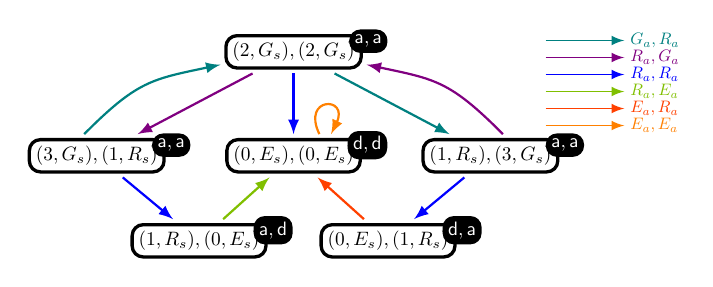
\begin{tikzpicture}[yscale=1.2, %
      gr/.style={green!50!blue}, %
      rg/.style={red!50!blue}, %
      rr/.style={blue}, %
      re/.style={green!50!orange}, %
      er/.style={red!50!orange}, %
      ee/.style={orange}, %
      ]

    \foreach \a/\hone/\perone/\htwo/\pertwo/\prop/\x/\y in { %
      s22gg/2/G_s/2/G_s/{a,a}/0/1.1,%
      s00/  0/E_s/0/E_s/{d,d}/0/0,%
      s31/  3/G_s/1/R_s/{a,a}/-2.5/0,%
      s13/  1/R_s/3/G_s/{a,a}/2.5/0,%
      s10/  1/R_s/0/E_s/{a,d}/-1.2/-0.9,%
      s01/  0/E_s/1/R_s/{d,a}/1.2/-0.9%
    }{ %
      \node[scale=0.7, outer sep=1mm,draw, very thick, rounded corners] (\a) at (\x,\y) {$(\hone,\perone), (\htwo,\pertwo)$};

      \node[fill=black, text=white, rounded corners, inner sep=1mm, scale=0.7, xshift=0.3mm, yshift=-2mm] at (\a.north east) {$\mathsf{\prop}$};
      }

      \foreach \from/\to/\lab/\wh in { %
        s22gg/s00/{rr}/left, s22gg/s31/{rg}/left, s22gg/s13/{gr}/right, %
        s31/s10/{rr}/left, %
        s13/s01/{rr}/left, %
        s10/s00/{re}/left,%
        s01/s00/{er}/right%
      }{ \draw[-latex,thick,\lab] (\from) -- (\to);
      }

      \foreach \from/\to/\out/\in/\loose/\lab/\wh in { %
        s00.40/s00.30/120/60/8/{ee}/above,%
        s31.120/s22gg.190/40/190/1.2/{gr}/right,%
        s13.60/s22gg.350/140/350/1.2/{rg}/left%
      }{%
        \draw[-latex,thick,\lab] (\from) to[out=\out,in=\in, looseness=\loose]  (\to); %
      }

      \begin{scope}[yshift=1.4cm]
      \foreach \col/\y/\lab in { %
        gr/1/{G_a,R_a}, rg/2/{R_a,G_a}, rr/3/{R_a,R_a}, %
        re/4/{R_a,E_a}, er/5/{E_a,R_a}, ee/6/{E_a,E_a}%
      }{ \draw[-latex, semithick, \col] (3.2,-0.18*\y) -- ++(1,0) node[right, scale=0.6] {$\lab$}; }
    \end{scope}
    \end{tikzpicture}
  \end{center}
 
\end{example}


A path in a model $\msys n$ is an infinite sequence of global states anc joint
actions $q^0\alpha^0q^1\alpha1\ldots$ such that $(q^i,\alpha^i,q^{i+1}) \in
\globalrel n$ for all $i \geq 0$. Given a global state $q$ in $\msys n$ we write
$\paths{q}$ for the set of all paths originating from $q$.
  
We express specifications for PNIS in an indexed and bounded variant of
Computation Tree Logic ($\ctl$), henceforth $\bictl$. The logic (i) introduces
indexed atomic propositions that are quantified over the agents of the concrete
system the formula in question is evaluated; and (ii) permits only the
construction of formulae whose evaluation can be realised on paths of bounded
lengths. The former extends $\ctl$ by allowing the formulation of properties
irrespective of the concrete system on which they are evaluated.  The latter
restrict $\ctl$ following the undecidability verification for unbounded
formulae~\cite{Akintunde+20}.

\begin{definition}
Given a  set $\atprop$ of atomic propositions and a set $\atvar$ of variables,
the $\bictl$  formulae are defined by the following BNF:
\[
  \varphi \;   ::= \; (p, v) \mid \varphi \lor \varphi \mid \varphi \land \varphi
  \mid AX^K \varphi \mid \forall v : \phi,
\]
where  $p \in \atprop$, $v \in \atvar$ and $k \geq  1$.
\end{definition}

The formula $AX^k \varphi$ is read as ``for all paths, $\varphi$ holds at the
$k$-th step''. We inductively abbreviate bounded until as
\begin{align*}
 A(\varphi U^1 \psi) &\triangleq \psi \lor (\varphi \land AX^1 \psi) \\
 A(\varphi U^k \psi) &\triangleq \psi \lor (\varphi \land AX^1 (A (\varphi U^{k-1} \psi)).
\end{align*}
with the meaning ``there is a path in which $\psi$ holds at some point in the
$k$ following steps and before then $\varphi$ is true along the path. 
% The dual
% until, prefixed by the universal operator, can be defined analogously.

A $\bictl$ formula is said to be a sentence if every variable appearing the
formula is in the scope of a universal quantifier. Hereafter we consider only
indexed $\bictl$ sentences of the form $\forall v_1 \ldots \forall v_m :
\varphi$, or, shortly, $\bictlspec$, where $v_i \in \atvar$ for $i \in
\set{1,\ldots,m}$ and $\varphi$ does not contain any universal quantifier.

We now define the satisfaction relation for $\bictl$ on the temporal models
associated with the concrete systems.

\begin{definition}[Satisfaction]
  \label{def:sat} 
  Given a model $\msys n$, a global state~$q^0$ and a $\bictl$ sentence
  $\bictlspec$ with $m \leq n$, the \emph{satisfaction} of $\varphi$ at $q$\nb{E: $q$ or $q^0$?},
  denoted $(\msys n, q) \models\varphi$, or simply $q \models \varphi$ when
  $\msys n$ is clear from the context, is defined as follows:
  \begin{description}
  \item[$q \models (p, a)$] \ iff \ $q^o \in \valuation n((p, a))$, for $p \in
  \atprop$ and $a \in \agents n$; 
  \item[$q \models \varphi \lor \psi$] \ iff \ $q \models \varphi$ or $q \models
  \psi$;
  \item[$q \models \varphi \land \psi$] \ iff \ $q \models \varphi$ and $q
  \models \psi$;
  \item[$q \models EX^k  \varphi$] \ iff  there is $\rho \in \paths{q}$ such
  that $\rho(k) \models \varphi$;
  \item[$q \models AX^k  \varphi$] \ iff for all $\rho \in \paths{q}$ we
  have that $\rho(k) \models \varphi$;
  \item[$q \models \bictlspec$] \ iff for all $h : \set{v_1, \ldots, v_m}
  \rightarrow \set{\ag 1, \ldots,\ag n}$ we have that $q \models 
  \varphi[v_1 \mapsto h(v_1), \ldots v_m \mapsto h(v_m)]$\nb{E: what is $h$? Would be good to explain it}
\end{description}
\end{definition}

A sentence $\bictlspec$ is said to be true in $\msys n$, denoted $\msys n
\models \bictlspec$ if $(\msys n, \globalinit n) \models \bictlspec$. The
sentence is said to be true in $\npis$, denoted $\npis \models \bictlspec$, if
$\bictlspec$ is true in every model induced by every concrete system
instantiated from $\npis$ with at least $m$ agents, i.e., $\forall n \geq m :
\msys n \models \bictlspec$.  The {\em parameterised verification problem} is to
check whether this holds.


\begin{definition}[Parameterised verification problem]
  Given an NPIS $\npis$ and a $\bictl$ sentence $\bictlspec$, determine whether
  $\npis \models \bictlspec$.
\end{definition}

  
  % Lomuscio, 2016b]. Given a set IND of indices, a set L AP
  % of local atomic propositions and a set G AP of global
  % atomic propositions, IACTLK\X formulae are defined by
  % the following BNF grammar:
  % φ ::= (p, v) | ¬(p, v) | q | ¬q | φ ∧ φ | φ ∨ φ | A(φU φ) |
  % A(φRφ) | Kiφ | ∀v : φ
  % where p ∈ L AP , q ∈ G AP , and v ∈ IND. The epis-
  % temic modality Kiφ is read as “agent i knows that φ”. The
  % temporal modality A(φU ψ) stands for “for all paths, at some
  % point ψ holds and before then φ is true along the path”; and
  % A(φRψ) denotes “for all paths, ψ holds along the path up to
  % and including the point when φ becomes true in the path”. An
  % IACTLK\X formula is said to be a sentence if every variable
  % appearing the formula is in the scope of a universal quantifier.
  % Hereafter we consider only indexed IACTLK\X sentences.
  % We now define the satisfaction relation.

  % We verify NIS against a bounded variant of a restricted
  % subset of ATL∗ (Alur, Henzinger, and Kupferman 2002),
  % drawing inspiration from Real Time Computation Tree
  % Logic (RTCTL) (Emerson et al. 1992). The satisfaction sta-
  % tus of the formulae expressible in our language depends only
  % on paths of a bounded length. This has been shown to be
  % practically relevant by enabling the efficient identification
  % of shallow bugs in a system’s execution (Biere et al. 2003;
  % Penczek, Wo´zna, and Zbrzezny 2002). In addition to this


  % practical consideration, our restriction to a bounded frag-
  % ment of ATL∗ follows the undecidability of the verification
  % problem for unbounded formulae (Akintunde et al. 2020a




%%% Local Variables:
%%% mode: latex
%%% fill-column: 79
%%% TeX-master: "../main"
%%% End:

\section{Parameterised Verification Procedure}
\label{sec:verification}
In this section we put forward a procedure for solving the parameterised
verification problem introduced in the previous section. For ease of
presentation we fix a PNIS $\pnis = \tuple{t, e, \ell}$, where $\ag t =
\tuple{\lstates t, \init t, \obs t, \acts t, \prot t, \tr t }$, $\ag e =
\tuple{\lstates e, \acts e, \prot e, \tr e }$, and a $\bictl$ sentence
$\bictlspec$ throughout the section. The verification procedure that we
introduce recasts the parameterised verification problem for $\pnis$ and
$\bictlspec$  to a (standard) verification problem for NIS $\pnis_{zo}$, which
we below define as a zero-one abstraction of the concrete systems generated from
$\pnis$,  and the $\bctl$ formula $\varphi[v_1 \mapsto 1, \ldots, v_m \mapsto
m]$.  We show that the satisfaction status of $\varphi[v_1 \mapsto 1, \ldots,
v_m \mapsto m]$ on $\pnis_{zo}$ determines the the satisfaction status of
$\bictlspec$ on $\pnis$. This enables us to use previously established
methodologies for the verification of NIS against $\bctl$~\cite{Akintunde+20b}
to solve the verification problem for PNIS.


We start by reducing the problem of checking the $\bictl$ sentence in question
to that of checking a $\bctl$ formula. This formula is any ground instantiation
of $\bictlspec$ which we fix to $\varphi[v_1 \mapsto 1, \ldots, v_m \mapsto m]$
and for brevity denote as $\varphi[m]$.


\begin{lemma}[Symmetry reduction]
\label{lemma:symmetry}
$\pnis \models \bictlspec$ iff $\pnis \models \varphi[m]$.
\end{lemma}
\begin{proof}
The lemma follows from the inherent symmetry present in systems comprising
homogeneous agents. The Appendix includes the full proof.
\end{proof}

We next construct the zero-one abstraction of the systems generated from
$\pnis$. The zero-one abstraction is a NIS comprising a zero-one agent, which is
an abstraction for arbitrarily many concrete agents, $m$ concrete agents, whose
<<<<<<< HEAD
local states determines the satisfaction status of the atomic propositions in
$\varphi[m]$ (see
=======
local states determine the satisfaction status of the atomic propositions in
$\varphi[v_1 \mapsto 1, \ldots, v_m \mapsto m]$ (see
>>>>>>> 80f46e43fa732afd4f55f01e124a28454ddbd83b
Definition~\ref{def:concreteystem}), and the environment. In other words, the
zero-one agent defined below encodes how an arbitrary number of agents may
interfere with the temporal evolution of the concrete agents $1, \ldots, m$.

\begin{definition}[Zero-one agent]
Given an agent template $\ag t = \tuple{\lstates t, \init t, \obs t,  \acts t,
\prot t, \tr t }$ over a set $\pers t$ of percepts and a set $\prvs t$ of
private states, its associated \emph{zero-one agent} is a tuple $\ag{zo} =
\tuple{\lstates{zo}, \init{zo}, \obs{zo}, \acts{zo}, \prot{zo}, \tr{zo}}$ over
sets $\pers{zo} = 2^{\pers t} \setminus \set{\emptyset}$ and $\prvs{zo}=
2^{\prvs t} \setminus \set{\emptyset}$ of percepts and private states, where:
\begin{itemize} 
    \item $\lstates{zo} = 2^{\lstates t} \setminus \set{\emptyset}$ is the set
    of abstract states. An abstract state represents the projection of global
    states in systems of any size onto a set.

    \item $\init{zo} = \set{\init t}$ is the unique initial abstract state.
    
    \item $\obs{zo} : \lstates{zo} \times \lstates e \rightarrow \per{zo}$ is
    abstract observation function. It maps pairs of abstract and environment
    states to sets of percepts, where each set includes the percepts that would
    be collectively generated in a global state represented by the abstract
    state. Formally, the observation function satisfies $\obs{zo}(l_{zo}, l_e) =
    \per{zo}$ if:
    \begin{itemize}
        \item for all $l_t \in l_{zo}$ we have that $\obs t(l_t, l_e) \in
        \per{zo}$;
        \item for all $\per t \in \per{zo}$ there is $l_t \in
        l_{zo}$ such that $\obs t(l_t, l_e) = \per t$.
    \end{itemize}

    \item $\acts{zo} = 2^{\lstates t \times \acts t} \setminus \set{\emptyset}$
    is the set of abstract actions. Analogously to abstract states, an abstract
    action represents the projection of joint actions, paired with the local
    states at which they are performed,  of arbitrarily many agents onto a set.

    \item $\prot{zo} : \lstates{zo} \rightarrow 2^{\acts{zo}} \setminus
    \set{\emptyset}$ is the abstract protocol. The protocol prescribes the sets
    of template actions that can be collectively performed at a global state
    represented by a given abstract state. It is defined as $$\prot{zo}(l_{zo})
    = \set{ \bigcup_{l_t \in l_{zo}} \set{l_t} \times A_{l_t} \mid A_{l_t} \in
    2^{\prot t(l_t)} \setminus \set{\emptyset}}.$$

    \item $\tr{zo} \colon \lstates{zo} \times \acts{zo} \times 2^{\acts t} 
    \times \acts e \rightarrow \prvs{zo}$ is the abstract transition function.
    The function determines the set of private states that the agents would
    collectively transition to in any global state represented by a given
    abstract state after they have performed a joint action represented by a
    given abstract action. It is s.t. $\tr{zo}(l_{zo}, \alpha_{zo}, A, \alpha_e)
    = \prv{zo}$ if the following hold:
    \begin{itemize}
        \item $\alpha_{zo} \in \prot{zo}(l_{zo})$; 
        \item for all $(l_t, \alpha_t) \in \alpha_{zo}$ we have that $\tr t(l_t,
        \alpha_t, A', \alpha_e) \in \prv{zo}$, where $A' = A \cup \set{\alpha'_t
        \mid (l'_t, \alpha'_t) \in \alpha_{zo} \text{ for some } l'_t})$;
        \item for all $\prv t \in \prv{zo}$, there is $(l_t, \alpha_t) \in
        \alpha_{zo}$ s.t. $\tr t(l_t, \alpha_t, A', \alpha_e) = \prv t$, where
        $A'$ is as in the above clause.  
    \end{itemize}
\end{itemize}
\end{definition}

The abstract  NIS comprised the zero-one agent and~$m$ concrete agents. It is a
tuple $\pnis_{zo} = \tuple{\set{1,\ldots,m,zo,e}, \globalinit{m}_{zo},
\valuation{m}_{zo}}$, where $\globalinit{m}_{zo} = \tuple{\init 1, \ldots, \init
m, \init{zo}, \init e}$ is the initial global state and $\valuation{m}_{zo} :
\atprop \times \set{1, \ldots, m } \rightarrow 2^{\globalstates{m}_{zo}}$ is the
concrete labelling function satisfying $q \in \valuation{m}_{zo}(p,a)$ iff
$\ls{a}{q} \in \tlabel a(p)$.  The global transition function is defined as in
Definition~\ref{def:globaltransition} but replacing $A$ in the environment
conditions in the first clause with $A = \set{\la{a}{q} \mid a \in
\set{1,\ldots,n}} \cup \la{zo}{q}$, similarly replacing~$A$ for the concrete
agents' conditions in the second clause, and adding analogous conditions for the
zero-one agent. Given the global transition function we can similarly associate
a model  $\masys m = \tuple{\aglobalstates m}$

We now establish a correspondence between the abstract models and the concrete
models. We show in particular that (i) the abstract model simulates every
concrete model with at least~$m+1$ agents; (ii) there is always a concrete model
with a sufficient number of agents that simulates the abstract model; and (iii)
a concrete models always simulates a smaller model. A model simulates another
model if every behaviour exhibited by the latter is also admitted by the former.
As specifications for PNIS are bounded, we consider simulation up to a bounded
number of steps as defined below.

\begin{definition}[Bounded simulation.]
A $b$-bounded simulation between two models $\mathcal M = \tuple{G, \it{ACT}, T,
\ell}$ and $\mathcal{M'} = \tuple{G', \it{ACT'}, T', \ell'}$  with initial
global states $\iota$ and $\iota'$ is inductively defined on $b \geq 0$ as
follows.
\begin{itemize}
    \item A relation $\sim_0 \subseteq G \times G'$ is  $0$-bounded simulation
    if $(\iota, \iota') \in sim_0$ and whenever $(q, q) \in \sim_0$, we have
    that $q \in \ell(p,a)$ implies that $q' \in \ell'(p, a)$, for any $p \in
    \atprop, a \in \mathbb N$.
    \item A relation $\sim_b \subseteq G \times G'$ is  $b$-bounded simulation
    if $(\iota, \iota') \in \sim_b$ and  whenever $(q, q') \in \sim_b$, the
    following conditions hold:
    \begin{enumerate}
    \item $(q, q') \in \sim_0$.
    \item If $(q, \alpha, q^1) \in T$ for a joint action $\alpha \in \it{ACT}$ and
    global state $q^1 \in G$, then there is a joint action
    $\alpha' \in \it{ACT}'$ and global state $g'^1$ such that
    $(g', \alpha', g'^1) \in T'$ and 
    $(q^1, q'^1) \in \sim_{b - 1}$.  
\end{enumerate}
\end{itemize}
\end{definition}

We say that a model $\mathcal{M'}$ simulates a model $\mathcal M$ up to~$b$ time
steps, denoted $\mathcal M \leq_b \mathcal{M'}$, if there is a $b$-bounded
simulation relation between $\mathcal M$ and $\mathcal{M'}$.  Universal $\bctl$
formulae are preserved from the simulating model to the simulated model and
existential $\bctl$ formulae are preserved from the simulated model to the
simulating model if their temporal depth is at most~$b$. 

\begin{theorem} Let $\mathcal M$ and $\mathcal M'$ be two models such $\mathcal
M \sim_b  \mathcal M'$. Then, the following hold.
\label{th:sim}
\begin{enumerate}
    \item If $\mathcal M' \models \varphi$ for a universal $\bctl$ formula
    $\varphi$ with $\td{\varphi} \leq b$, then $\mathcal M \models
    \varphi$.
    \item If $\mathcal M \models \varphi$ for an existential $\bctl$ formula
    $\varphi$ with $\td{\varphi} \leq b$, then $\mathcal M' \models
    \varphi$.
\end{enumerate}
\end{theorem}
\begin{proof}[Proof Sketch.]
The result is established in~\cite{ClarkeGrumbergLong94} for arbitrary Kripke
structures and unbounded $\ctl$ formulae and simulations. Since $\bctl$ formulae
are evaluated up to a bounded temporal depths, they are preserved under bounded
simulations.
\end{proof}

We can now show that the simulation results pertaining to the abstract and
concrete model.  We start by showing that the abstract model simulates every
concrete model with at least~$m+1$ agents.

\begin{theorem}
\label{th:ab-concr-sim}
$\msys n \leq_b \masys m$ for any $n \geq m+1$ and $b \geq 0$.
\end{theorem}
\begin{proof}
The proof proceeds by induction on~$b$ and it is included in the Appendix.
\end{proof}

Irrespective of the temporal depth of the specification under
analysis there is always a concrete model that simulates the abstract model up
to that depth.

\begin{theorem}
\label{th:concr-ab-sim}
There is $n \geq m+1$ such that $\masys m \leq_b \msys n$ for any $b \geq 0$.
\end{theorem}
\begin{proof}
The proof proceeds by induction on~$b$ and it is included in the Appendix.
\end{proof}


Every concrete model simulates every smaller concrete models.

\begin{theorem}
\label{th:concr-sim}
For every $n > m$ and $n' > n$ we have that $\msys n \leq_b \msys{n'}$ for any
$b \geq 0$.
\end{theorem}
\begin{proof}
The proof proceeds by having every additional agents in $\msys{n'}$ to mimic
agent~1 in $\msys n$ and it is included in the Appendix.
\end{proof}

The above results enable the derivation of verification procedures for solving
the parameterised verification and emergence identification problem. In the case
of universal formulae the emergence identification procedure simply concerns
checking the abstract model and the parameterised verification procedure 
additionally involves checking a single concrete model against the formula in
question.

\begin{corollary}
\label{cor:universal}
If $\varphi[m]$ is a universal $\bctl$ formula and we have that $\masys m
\models  \varphi[m]$, then the following hold:
\begin{itemize}
    \item  If $\masys m \models \varphi[m]$, then $m + 1$ is an emergence
    threshold for $\bictlspec$. Otherwise, there is no emergence threshold for
    $\bictlspec$.
    \item $\masys m \models \varphi[m] \land \msys m \models \varphi[m]$ iff
    $\pnis \models \bictlspec$.
\end{itemize}
\end{corollary}
\begin{proof}
To prove the first clause assume that $\masys m \models \varphi[m]$. By
Theorem~\ref{th:ab-concr-sim} we have that $\msys n \models \varphi[m]$ for
every $n \geq m+1$. Lemma~\ref{lemma:symmetry} gives that  $\msys n \models
\bictlspec$ for every $n \geq m+1$. Hence, $m+1$ is an emergence threshold for
$\bictlspec$. If otherwise we have that  $\masys m \not \models \varphi[m]$,
then by Theorem~\ref{th:concr-ab-sim} there is $n \geq m+1$ such that $\msys n
\not \models \varphi[m]$. Theorem~\ref{th:concr-sim} additionally gives that
$\msys{n'} \not \models \varphi[m]$ for every $n' \geq n$. Thus, from
Lemma~\ref{lemma:symmetry}, we obtain that $\msys n' \not \models \bictlspec$
for every $n' \geq n$, therefore there is no emergence threshold for
$\bictlspec$.

To prove the second clause assume that $\masys m \models \varphi[m]$ and $\msys
m \models \varphi[m]$. By Theorem~\ref{th:ab-concr-sim} we have that $\msys n
\models \varphi[m]$ for every $n \geq m$. From Lemma~\ref{lemma:symmetry} we
obtain that $\msys n \models \bictlspec$ for every $n \geq m$, thus $\pnis
\models \bictlspec$. If otherwise $\masys m \not \models \varphi[m]$ or $\msys m
\not \models \varphi[m]$, then by Theorem~\ref{th:concr-ab-sim}, there is $n
\geq m$ such that $\msys n \not \models \varphi[m]$.  From
Lemma~\ref{lemma:symmetry} we obtain that there is $n \geq m$ such that $\msys n
\not \models \bictlspec$. Consequently, $\pnis \not \models \bictlspec$.
\end{proof}

So every universal $\bctl$ formula satisfied by the abstract model
and the concrete model of $m$ agents is also satisfied by the parameterised
system. This also implies that~$m$ is an emergence threshold for the formula.

Theorem~\ref{th:concr-sim} additionally enables the derivation of a simple
procedure for the verification of existential properties.

\begin{corollary}
\label{cor:existential}
If $\varphi[m]$ is an existential $\bictl$ formula with temporal depth $b$ and  $n
= \min_i \left( \masys m \leq_b \msys i \right)$, then the following hold:
\begin{itemize}
\item If $\msys n \models \varphi[m]$, then $n$ is an emergence threshold for
$\bictlspec$. Otherwise, there is no emergence threshold for $\bictlspec$.

\item $\msys i \models \bictlspec$, for all $i \in \set{m, \ldots, n}$, iff
$\pnis \models \bictlspec$.
\end{itemize}
\end{corollary}
\begin{proof}
To prove the first clause assume that $\msys n \models \varphi[m]$. By
Theorem~\ref{th:concr-sim} we have that $\msys{n'} \models \varphi[m]$ for every
$n' \geq n$. Lemma~\ref{lemma:symmetry} gives that  $\msys{n'} \models
\bictlspec$ for every $n' \geq n$. Hence, $n$ is an emergence threshold for
$\bictlspec$. If otherwise we have that  $\msys n \not \models \varphi[m]$, then
by Theorem~\ref{th:concr-ab-sim} it follows  that $\masys m \not \models
\varphi[m]$, hence, by Theorem~\ref{th:ab-concr-sim}, $\msys n' \not \models
\varphi[m]$ for every $n' \geq m+1$.  Thus, from Lemma~\ref{lemma:symmetry}, we
obtain that $\msys{n'} \not \models \bictlspec$ for every $n' \geq m + 1$,
therefore there is no emergence threshold for $\bictlspec$.

To prove the second clause assume that $\msys i \models \varphi[m]$ for every $i
\in \set{m,\ldots,n}$.  By Theorem~\ref{th:concr-sim} we have that $\msys{i}
\models \varphi[m]$ for every $i \geq m$. Lemma~\ref{lemma:symmetry} gives that
$\msys{i} \models \bictlspec$ for every $i \geq m$. Hence, $\pnis \models
\bictlspec$.  If otherwise there is $i \in \set{m, \ldots, n}$ such that $\msys
i \not \models \varphi[i]$, then, by Lemma~\ref{lemma:symmetry}, we have that
$\msys i \not \models \bictlspec$, which trivially implies that $\pnis \not
\models \bictlspec$.
\end{proof}
% \begin{proof}[Proof Sketch]
%     The proof is analogous to the proof of Corollary\ref{cor:universal}.
% \end{proof}

In summary, Corollaries~\ref{cor:universal} and~\ref{cor:existential} provide
constructive, sound and complete methodologies for checking universal ans
existential specifications for PNIS.  For universal properties, verification can
be conducted by constructing and checking the abstract model and the concrete
model with~$m$ agents, where $m$ is the the number of index variables in the
specification in question. The specification is satisfied by the abstract and
concrete models iff the specification is satisfied in general for any number of
agents.  The satisfaction of the specification by the abstract model is also
connected by biconditional implication with the existence of an emergent
threshold for the specification. For existential properties, verification can be
performed by checking all concrete models up to the concrete model that
simulates the abstract model. The specification is satisfied by all these
concrete models iff the specification is satisfied in general for any number of
agents.   The satisfaction of the specification by the concrete model that
simulates the abstract model is also connected by biconditional implication with
the existence of an emergent threshold for the specification. 



% \begin{corollary}
% If $\bictlspec$ is an existential $\bictl$ sentence with temporal depth $b$, $n
% = \min_i \left( \masys m \leq_b \msys i \right)$, and we have that $\msys n
% \models \bictlspec$, then $n$ is an emergence threshold for $\bictlspec$.
% \end{corollary}



% It follows that if the abstract model does not satisfy the formula in question
% then the parameterised system does not satisfy the formula either. Moreover,
% since the abstract model also simulates said concrete model and as the
% simulation relation is transitive, it follows that the concrete model simulates
% every bigger model, hence there is no emergence threshold for the specification.


% \begin{corollary}
% If $\varphi[m]$ is a universal $\bctl$ formula and we have that $\masys m \not
% \models  \varphi[m]$, then it follows that (i) $\pnis \not \models \bictlspec$
% and (ii) there is no emergence threshold for $\bictlspec$.
% \end{corollary}
% \begin{proof}
% The result follows from Theorem~\ref{th:ab-sim}, Theorem~\ref{th:concr-sim} and
% Lemma~\ref{lemma:symmetry}.
% \end{proof}

\section{Evaluation}

In this section we present an evaluation of the parameterised verification
procedure described in Section~\ref{sec:verification} for the guarding game
presented in Example~\ref{ex:agent-template}.


The guarding game is an instance of a social dilemma game
\cite{LeiboZLMG17}. Such games are characterised by an intrinsic tension
between individual and collective goals.

We used reinforcement learning to learn the neural observation function, where
the agents have been given instantaneous rewards when ...

deep Q-learning..

The resulting NN has 1 hidden layer of .. neurons and ReLU activation function.



Given the neural network implementing the observation function, we 
implemented an agent template and a zero-one agent for the guarding game. We
then used the \venmas toolkit developed for verification of
NISs~\cite{Akintunde+20b} to verify $\bctl$ properties checking whether it is
possible for a colony of agents to survive after a number of time steps.

We assume that $M_h = 4$, $G_r = -2$, $R_r = 1$ and $U_r = -3$. 

Assume the set $\atprop$ and the labelling function $\ell$ as in
Example~\ref{ex:pnis}. We evaluate the zero-one NIS
$\pnis_{zo} = \tuple{\set{1,\ldots,m,zo,e}, \globalinit{m}_{zo}, \valuation{m}_{zo}}$
against two specifications:
$\varphi^k_1 = EX^k \bigwedge_{i=1}^m(\mathsf{a},i)$,
expressing that there is a way to choose agents' actions from those available
to them so that all three agents are alive after $k$ time steps, and
$\varphi^k_2 = AX^k (\mathsf{a},1) \land (\mathsf{a},2) \land (\mathsf{a},3)$,
expressing that for all possible evolutions after $k$ time steps all three
agents are alive.

The experiments have been performed on a standard PC running Ubuntu 22.04 with
16GB RAM and processor Intel(R) Core i5-4460 CPU @ 3.20GHz. We relied on Gurobi
v9.5.1 to solve MILP \cite{Gurobi+16a}.



\begin{table}
\centering
\begin{tabular}{ccrcrc}
  \toprule
  & $k$ & \multicolumn{2}{c}{$m = 2$} & \multicolumn{2}{c}{$m = 3$}  \\\midrule
  $\varphi_1^k$ & 1 &     0.76s & True    &     2.03s & True   \\
               & 2 &     4.53s & True    &    20.06s & True   \\
               & 3 &     8.64s & True    &    31.78s & True   \\
               & 4 &    28.48s & True    &   Timeout & --     \\
  \midrule
  $\varphi_2^k$ & 1 &     0.71s & False   &     1.85s & False  \\
               & 2 &     3.57s & False   &    15.93s & False  \\
               & 3 &     9.16s & False   &    32.78s & False  \\
               & 4 &    13.31s & False   &    47.20s & False  \\

\bottomrule
\end{tabular}
  % \caption{ Verification times for \guard{m} against properties $\varphi_{1}^{k}$
  %   and $\varphi_{2}^{k}$ for various $k$ and $h_\init$.  Grey cells indicate a
  %   % \texttt{\greyc} result, otherwise a \texttt{True} result was obtained.
  %   % Dashes indicate a \timeout hour timeout.
  % }
  \label{tab:results}
\end{table}



%%% Local Variables:
%%% mode: latex
%%% fill-column: 79
%%% TeX-master: "../main"
%%% End:

\section*{Appendix}
\subsection*{Proof of Lemma 1} 
We prove the symmetry reduction Lemma which we restate here for convenience:
\begin{customlemma}{1}
$\pnis \models \bictlspec$ iff $\pnis \models \varphi[v_1 \mapsto 1, \ldots, v_m
\mapsto m]$.
\end{customlemma}
\begin{proof}
Let $n \in \mathbb N$ such that $n \geq m$ be arbitrary. We show that $\msys n
\models \bictlspec$ iff $\msys n \models \varphi[v_1 \mapsto 1, \ldots, v_m
\mapsto m]$. The Lemma then follows.

$\boldsymbol{(\Longleftarrow)}$ For the right to left direction assume that $\msys n \models
\bictlspec$. Then, by the definition of satisfaction of $\bictl$
(Definition~\ref{def:sat}), we have that for all $h: \set{v_1, \ldots, v_m}
\rightarrow \set{1,\ldots,n}$,  it holds that $\msys n \models \varphi[v_1
\mapsto h(v_1), \ldots, v_m \mapsto h(v_m)]$.  Hence, $\msys n \models
\varphi[v_1 \mapsto 1, \ldots, v_m \mapsto m]$.


$\boldsymbol{(\Longrightarrow)}$ For the left to right direction assume that $\msys n \models
\varphi[v_1 \mapsto 1, \ldots, v_m \mapsto m]$. Let $I = \set{i_1, \ldots, i_m}
\in \set{1, \ldots, n}^m$ be an arbitrary set of $m$ distinct integers within
$\set{1,\ldots,n}$.  Consider $\sigma : \set{1, \ldots, n} \rightarrow \set{1,
\ldots, n}$ be a bijective mapping such that $\sigma(j) = i_j$ for all $j$ with
$1 \leq j \leq m$. For a global state $q$, denote by $\pi(q)$ the global state
obtained by replacing every $i$-th local state in $q$ with the $\sigma(i)$-th
local state in $q$. Similarly, for a joint action $\alpha$, denote by
$\pi(\alpha)$ the joint action obtained by replacing every $i$-th local action
in $\alpha$ with the $\sigma(i)$-th local action in $\alpha$. Then, by the
definition of the global transition function
(Definition~\ref{def:globaltransition}), we have that $\globaltr n(q, \alpha) =
q'$  iff $\globalrel n(\pi(q), \pi(\alpha)) = \pi(q')$.  Hence,  $(q, \alpha,
q') \in \globalrel n$ iff $(\pi(q), \pi(\alpha), \pi(q')) \in \globalrel n$.
Therefore, ($\msys n, q) \models  \varphi[v_1 \mapsto 1, \ldots, v_m \mapsto m]$
iff ($\msys n, \pi(q)) \models  \varphi[v_1 \mapsto \pi(1), \ldots, v_m \mapsto
\pi(m)]$. So, by the initial assumption,  it follows that ($\msys n,
\pi(\globalinit{n})) \models  \varphi[v_1 \mapsto \pi(1), \ldots, v_m \mapsto
\pi(m)]$. As $\pi(\globalinit{n}) = \globalinit{n}$, we have that ($\msys n,
\globalinit{n}) \models  \varphi[v_1 \mapsto \pi(1), \ldots, v_m \mapsto
\pi(m)]$. Since the set of indices $I$ was arbitrary, we conclude that $\msys n
\models \bictlspec$.  \end{proof}


\subsection*{Formal definition of the abstract global transition function} In the
following we give the full formal definition of the abstract transition function.
\begin{definition}
  \label{def:globaltransition}
  The {\em global transition function} $\globaltr{m}_{zo} : \globalstates{m}_{zo}
  \times \globalacts{m}_{zo} \rightarrow \globalstates{m}_{zo}$ of the zero-one
  system $\sys{m}_{zo}$ satisfies $\globaltr{m}_{zo}(q, \alpha) = q'$ iff the
  following hold:
  \begin{itemize}
    \item $\la{e}{\alpha} \in \prot{e}({\ls{e}{q}})$ and $\tr e(\ls{e}{q},
    \la{e}{q}, A) = q'$, where
    $A = \set{\la{a}{q} \mid a \in \set{1,\ldots,n}} \cup
\la{zo}{q}$.
    \item For all $a \in \set{1,\ldots,m, \it{zo}}$, we have that
    $\la{a}{\alpha} \in \prot{a}(\ls{a}{q})$, $\tr a (\ls{a}{q}, \la{i}{\alpha},
    A, \la{e}{\alpha}) = \lprv{a}{q'}$, where  $A = \set{\la{a}{q} \mid a \in
    \set{1,\ldots,n}} \cup \la{zo}{q}$, and $\obs
    a((\lprv{a}{q'},\lper{a}{q}),\ls{e}{q'}) = \lper{a}{q'}$.
  \end{itemize}
\end{definition}





\subsection*{Proof of Theorem 1}
\begin{customthm}{1}
$\msys n \leq_b \masys m$ for any $n \geq m+1$ and $b \in \mathbb N$.
\end{customthm}
\begin{proof}
Let $n \geq m+1$. We show that $\msys n
\leq_b \masys m$ for any $b \geq 0$.
 Define $\gamma_n
\colon \globalstates n \rightarrow \aglobalstates m$ to map concrete states in
$\msys n$ to abstract states in $\masys m$ as follows:
\begin{align*}
  \gamma_n(q) =  \langle &\ls{1}{q}, \ldots, \ls{m}{q}, \\
  &\set{\ls{i}{q} \mid i \in \set{m + 1, \ldots, n}}, \\
  &\ls{e}{q}  \rangle.
\end{align*}

We show by induction on $b$ that $\sim_b = \set{(q, \gamma_n(q)) \mid q \in
\globalstates n }$ is a $b$-bounded simulation relation between $\msys n$ and
$\masys m$. 


{\bf Base step.} For the base step, let $b = 0$ and $(q, \abstate) \in \sim_0$
be arbitrary. As $\gamma_n$ preserves the local states of the agents $1, \ldots,
m$, we have that $q \in \valuation n(p, a)$ implies that $\abstate \in
\avaluation(p, a)$ for any $p \in \atprop$ and $a \in \set{1, \ldots, m}$, thus
$\sim_0$ is $0$-bounded simulation between $\msys n$ and $\masys m$.  

{\bf Inductive step.} For the inductive step assume that for any $b >0$,
$\sim_b$ is a $b$-bounded simulation between $\msys n$ and $\masys m$. We show
that $\sim_{b+1}$ is a $(b+1)$-bounded simulation relation  between $\msys n$
and $\masys m$.  As $\sim_{b-1} = \sim_0$, $\sim_{b-1}$ satisfies the first
condition a condition of a bounded simulation relation. To show that it
satisfies the second condition, let $(q, \abstate) \in sim_{b+1}$ be arbitrary
and assume that $(q, \alpha, q') \in \globalrel n$ for some joint action
$\alpha$ and global state $q'$. We need to show that there is an abstract joint
action $\abaction$ and an abstract global state $\abstatep$ such that
$(\abstate, \abaction, \abstatep) \in \aglobalrel m$ and $(q', \abstatep) \in
\sim_b$.  Define $\delta_n \colon \globalacts n \rightarrow \aglobalacts m$ to
map joint actions in $\msys n$ to joint actions in $\masys m$ as follows:
\begin{align*}
  \delta_n(\alpha) =  \langle &\la{1}{q}, \ldots, \la{m}{q}, \\
  &\set{\la{i}{q} \mid i \in \set{m + 1, \ldots, n}}, \\
  &\la{e}{q}  \rangle.
\end{align*}
Let $\abaction = \delta_n(\alpha)$. By the definition of the abstract protocol
function we have that $\abaction \in \prot{zo}(\abstate)$. So $(\abstate,
\abaction, \abstatep) \in \aglobalrel m$, where $\abstatep = \aglobaltr m
(\abstate, \abaction)$. By the definition of the concrete and abstract local
transition functions, and since the set $\set{\la{i}{\alpha} \mid i \in
\set{1,\ldots,n}}$ of actions in $\alpha$ equals the set $\set{\la{i}{q} \mid i
\in \set{1,\ldots,m}} \cup \set{\alpha_t \mid \exists l_t \colon (l_t, \alpha_t)
\in \la{zo}{\abaction}}$ of actions in $\abaction$, we have that $\ls{i}{q'} =
\ls{i}{\abstate}$ for $i \in \set{1,\ldots,m}$, and $\set{\ls{i}{q'} \mid i \in
\set{m+1,\ldots,n}} = \ls{zo}{\abstate'}$.  Therefore $(q', \abstatep) \in
\sim_b$ as required.

We have thus proven that for any $b \geq 0$, $\sim_b = \set{(q, \gamma_n(q))
\mid q \in \globalstates n }$ is a $b$-bounded simulation relation between
$\msys n$ and $\masys m$.  As by the definitions of the initial global states of
abstract and concrete models, we have that $(\globalinit{n}, \aglobalinit{,})
\in \sim_b$ we have that $\msys b \leq b \masys n$ for any $b \geq 0$.

\end{proof}


\subsection*{Proof of Theorem 2}
\begin{customthm}{2}
There is $n \geq m+1$ such that $\masys m \leq_b \msys n$ for any $b \geq 0$.
\end{customthm}

\begin{proof}

The proof of the Theorem is by induction on~$b$. For $n \geq m+1$,  define
$\gamma_n \colon \globalstates n \rightarrow \aglobalstates m$ to map concrete
states in $\msys n$ to abstract states in $\masys m$ as follows:
\begin{align*}
  \gamma_n(q) =  \langle &\ls{1}{q}, \ldots, \ls{m}{q}, \\
  &\set{\ls{i}{q} \mid i \in \set{m + 1, \ldots, n}}, \\
  &\ls{e}{q}  \rangle.
\end{align*}

{\bf Base step.} For the base step, let $b = 0$ and $n = m+1$. Define $$\sim_0 =
\set{(\abstate, q) \mid \abstate \in \aglobalstates{m}, q \in
\aglobalstates{m+1}, \gamma_{m+1}(q) = \abstate}.$$ As $\gamma_{m+1}$ preserves
the local states of the agents $1, \ldots, m$, we have that $\abstate \in
\avaluation m(p, a)$ implies that $q \in \valuation{m+1}(p, a)$ for any $p \in
\atprop$ and $a \in \set{1, \ldots, m}$, thus  $\sim_0$ is $0$-bounded
simulation between $\masys m$ and $\msys{m+1}$. Therefore, since
$(\aglobalinit{m}, \globalinit{m+1}) \in \sim_0$, we what that $\masys m \leq_0
\msys n$. 

{\bf Inductive step.} For the inductive step, assume that for each $i \in
\set{1, \ldots, b}$ there is $n \geq m + 1$ such that $\masys m \leq_b \msys n$
by means of relation $\sim_i$. We show that there is $n' \geq n$ such that
$\masys m \leq_{b+1} \msys{n'}$. Let $|\prot t| = \max \set{|\prot t(l_t)| \mid
l_t \in \lstates{t}}$ and  $n' = m + n * |\prot t|$.  Define the following
relations $\sim_i \subseteq \aglobalstates{m} \times \globalstates{n'}$ between
the abstract states in $\aglobalstates{m}$ and the global states in $\msys{n'}$:

\begin{itemize}

  \item  $\sim'_0 = \set{(\abstate, q) \mid  q_{ab \rightarrow m} =
  \projection{q}{m} [m]}$, where $q_{ab \rightarrow m}$ and $\projection{q}{n}$
  is the projection of $q_{ab}$ and $q$ onto the first~$m$ agents, e.g.,
  $\projection{q}{m} = \tuple{\ls{1}{q}, \ldots, \ls{m}{q}, \ls{e}{q}}$.


  \item for $i \in \set{1, \ldots, b + 1}$, we have that $(\abstate, q) \in
  \sim'_i$ if:
  \begin{itemize}
    \item  $(\abstate,\projection{q}{n}) \in \sim_{i-1}$, and 
    \item  for $j \in [n]$ and $k \in [|\prot t|]$, 
    $\ls{m + (j - 1) * |\prot t| + k}{q} = \ls{j}{q}$.
  \end{itemize}
\end{itemize}

We show that for every $x \in \set{0, \ldots, b+1}$, $\sim'_x$ is an $x$-bounded
simulation between $\masys m$ and $\msys{n'}$. We have three cases.

\begin{itemize}
  \item Case 1: $x=0$.  Since  $q_{ab \rightarrow m} = \projection{q}{m}$, we have that
  $q \in \avaluation m(p, a)$ implies that $q \in \valuation n (p, a)$ for any
  $p \in \atprop$ and $a \in [m]$, thus $\sim'_0$ is a $0$-bounded simulation
  between $\masys m$ and $\msys{n'}$.


  \item Case 2: $x = 1$.  By the definition of $\sim'_1$ we have
  that $(\abstate, \projection{q}{n}) \in \sim_{0}$, 
  thus  $q \in \avaluation m(p, a)$ implies that $\projection{q}{n} \in
  \valuation n (p, a)$ for any $p \in \atprop$ and $a \in [m]$. Hence, by the
  definition of the valuation function, we have that $q_{ab \rightarrow m} =
  \projection{q}{m}$, thus $(\abstate, q') \in \sim'_0$, so $\sim'_1$
  satisfies the first condition of bounded simulation. 


  To show that it satisfies the second condition, assume that $(\abstate,
  \abaction, \abstatep) \in \aglobalrel m$ for some abstract joint action
  $\abaction$ and abstract global state $\abstatep$. We need to show that there
  is a joint action $\alpha$ and a  global state $q'$ such that $(q, \alpha, q')
  \in \globalrel{n'}$ and $(\abstatep, q') \in \sim'_0$. Define $\alpha$ as
  follows:

  \begin{itemize}
    \item $\la{i}{\alpha} = \la{i}{\abaction}$, for $i \in [m]$.
    \item  for $i \in [n]$, consider the set $\set{a_t \mid (\ls{m + (i - 1) *
    |\prot t| + 1} {q},\alpha_t) \in \la{zo}{\abaction}}$ of template actions
    that are paired with the template state of the $(m + (i-1) + 1)$-the agent
    in the action of the zero-one agent. Assume an ordering $\alpha_1, \ldots,
    \alpha_j$ of this set and define
    \begin{itemize}
    \item  $\la{m + (i -1) * |\prot t| + k}{\alpha} = \alpha_k$  for $k \in [j]$.
    \item $\la{m + (i-1) * |\prot t| + k}{\alpha} = \alpha_1$ for $k \in
    \set{j+1, \ldots, |\prot t|}$.
    \end{itemize}
  \end{itemize}
  By the definition of $\alpha$ we have that $\la{i}{\alpha} \in \prot
  i(\ls{i}{q})$ for every $i \in [n']$. So $(q, \alpha, q') \in \globalrel
  {n'}$, where $q' = \globaltr{n'} (q, \alpha)$. By the definition of the
  concrete and abstract local transition functions, and since the set
  $\set{\la{i}{\alpha} \mid i \in [n']}$ of actions in $\alpha$ equals the set
  $\set{\la{i}{q} \mid i \in \set{1,\ldots,m}} \cup \set{\alpha_t \mid \exists
  l_t \colon (l_t, \alpha_t) \in \la{zo}{\abaction}}$ of actions in $\abaction$,
  we have that $q_{ab \rightarrow m} = \projection{q}{m}$, therefore
  $(\abstatep, q') \in \sim'_0$, as required. 


  \item Case 3: $x \in \set{2, \ldots, b+1}$.   By the definition of $\sim'_x$
  we have that $(\abstate, \projection{q}{n}) \in \sim_{x-1}$. By the definition
  of bounded simulation it follows that $(\abstate, \projection{q}{n}) \in
  \sim_0$, thus  $q \in \avaluation m(p, a)$ implies that $\projection{q}{n} \in
  \valuation n (p, a)$ for any $p \in \atprop$ and $a \in [m]$. Hence, by the
  definition of the valuation function, we have that $q_{ab \rightarrow m} =
  \projection{q}{m}$, thus $(\abstate, q') \in \sim'_0$, so $\sim'_{x}$
  satisfies the first condition of bounded simulation. 


  To show that it satisfies the second condition, assume that $(\abstate,
  \abaction, \abstatep) \in \aglobalrel m$ for some abstract joint action
  $\abaction$ and abstract global state $\abstatep$. We need to show that there
  is a joint action $\alpha$ and a  global state $q'$ such that $(q, \alpha, q')
  \in \globalrel{n'}$ and $(\abstatep, q') \in \sim'_{x-1}$. Since $(\abstate,
  \projection{q}{n}) \in \sim_{x-1}$, we have that there is a joint action
  $\beta$ and a global state $r$ such that $(\projection{q}{n}, \beta, r) \in
  \globalrel n$ and $(\abstate, r) \in \sim_{x-2}$. Define a joint action
  $\alpha \in \globalacts{n'}$ such that
  
  \begin{itemize}
    \item for $i \in [n]$, $\la{i}{\alpha} = \la{i}{\beta}$, 
    \item  for $i \in \set{0, \ldots, n-1}$ and $j \in [|\prot t| -  1]$, $\la{n +
    i * |\prot t| + j}{\alpha} = \la{i}{\beta}$.
  \end{itemize}

  By the definition of $\alpha$, we have that $(q, \alpha, q')  \in
  \globalrel{n'}$ for a global state $q'$ that satisfies

  \begin{itemize}
    \item  $(\abstate,\projection{q'}{n}) \in \sim_{b-1}$, and 
    \item  for $j \in \set{0, \ldots, n-1}$ and $k \in [|\prot t| -  1]$, 
    $\ls{n + j * |\prot t| + k}{q'} = \ls{j}{q'}$.
  \end{itemize}

  It follows that $(q, \alpha, q') \in \sim'_{x-1}$. Consequently, $\sim'_{x}$
  is an $x$-bounded simulation between $\masys m$ and $\msys{n'}$.

\end{itemize}

We have thus proven that for every $x \in \set{0, \ldots, b+1}$, $\sim'_x$ is an
$x$-bounded simulation between $\masys m$ and $\msys{n'}$.  As by the
definitions of the initial global states of abstract and concrete models, we
have that $(\aglobalinit{m}, \globalinit{n'}) \in \sim'_{b+1}$ we have that
$\masys m \leq_{b+1} \msys{n'}$.

\end{proof}



% We say that $\msys n$ and $\masys m$ are {\em $b$-bounded bisimiulation
% equivalent} models if there is a $b$-bounded bisimiulation relation $\sim_b$
% between $\msys n$ and $\masys n$  such that $(\globalinit n, \aglobalinit m) \in
% \sim_b$.

% where $\projection{q}{n} =
%   \tuple{\ls{1}{q}, \ldots, \ls{n}{q}, \ls{e}{q}}$ is the projection of $q$ to
%   the first~$n$ agents,  and 



% \begin{lemma} 
%   \label{lemma:lifting}
%   Let $m \in \mathbb{N}$, $n \geq m$ and $n' > n$. If $\sim_b = \set{\tuple{q,
%   \gamma_n(q)} \mid q \in \globalstates n}$ is a $b$-bounded bisimulation
%   relation between   $\msys n$ and $\masys{m}$, then the relation 
%   $$
%   \sim'_b = \set{(q, \gamma_{n'}(q)) \mid q \in \globalstates{n'}, 
%   \exists r \in \globalstates{n} \colon (r, \gamma_{n'}(q)) \in \sim_b}
%  $$
%   % \subseteq \globalstates{n'} \times \aglobalstates{m}$ satisfying $$(q,
%   % \abstate) \in \sim'_b \text{ iff } (\projection{q}{n}, \abstate) \in \sim_b$$ 
%   is a $b$-bounded bisimulation relation between $\msys{n'}$ and $\masys{m}$.
% \end{lemma}
% \begin{proof}

% Assume that $\sim_b$ is a $b$-bounded bisimulation relation between  $\msys n$
% and $\masys{m}$. We show that the relation $\sim'_b$ is a $b$-bounded
% bisimulation relation between  $\msys{n'}$ and $\masys{m}$. Let $(q, \abstate)
% \in \sim'_b$ be arbitrary. We need to show that $(q, \abstate)$ satisfies
% conditions 1-3 of Definition~\ref{def:bounded-bisimulation}.   By the definition
% of $\sim'$ there is a global state $r \in \globalstates{n}$ such that $(r,
% \gamma_{n'}(q)) \in \sim_b$.



% \begin{itemize}

%   \item[] Condition 1. Assume that $q \in \valuation{n'}(p,a)$ for some $p \in
%   \atprop$, $a \in \set{1, \ldots, m}$.  As  $\abstate = \gamma_{n'}(q)$ and
%   $\gamma_{n'}$ preserves the local states of the agents $1, \ldots, m$, we have
%   that $q \in \valuation{n'}(p,a)$ iff  $\abstate \in \avaluation m(p, a)$.

%   \item[] Condition 2. Assume that $(q, \alpha, q') \in \globalrel{n'}$ for a
%   joint action $\alpha$ and global state $q'$.  We need to show that there is  a
%   joint abstract action $\abaction$ and an abstract global state $\abstatep$
%   such that $(\abstate, \abaction, \abstatep) \in \aglobalrel m$ and $(q',
%   \abstatep) \in \sim'_{b-1}$.  
  
%   Let $\abaction = \delta_{n'}(\alpha)$. By the definition of the abstract
%   protocol function we have that $\abaction \in \prot{zo}(\abstate)$. So
%   $(\abstate, \abaction, \abstatep) \in \aglobalrel m$, where $\abstatep =
%   \aglobaltr m (\abstate, \abaction)$. By the definition of the concrete and
%   abstract local transition functions, and since the set $\set{\la{i}{\alpha}
%   \mid i \in \set{1,\ldots,n'}}$ of actions in $\alpha$ equals the set
%   $\set{\la{i}{q} \mid i \in \set{1,\ldots,m}} \cup \set{\alpha_t \mid \exists
%   l_t \colon (l_t, \alpha_t) \in \la{zo}{\abaction}}$ of actions in $\abaction$,
%   we have that $\ls{i}{q'} = \ls{i}{\abstate}$ for $i \in \set{1,\ldots,m}$, and
%   $\set{\ls{i}{q'} \mid i \in \set{m+1,\ldots,n'}} = \ls{zo}{\abstate'}$.
%   Therefore $\gamma_{n'}(q') =  \abstatep$. 

%   Now as $(r, \abstate) \in \sim_b$, there is a joint action $\beta$ such that
%   $(r, \beta, r') \in \globalrel{n}$ and $(r', \abstatep) \in \sim_{b-1}$. As
%   $\abstatep = \gamma_{n'}(q')$, we have that $(q', \abstatep) \in \sim'_{b-1}$,
%   as required.

%   \item Condition 3. Assume that $(\abstate, \abaction, \abstatep) \in
%   \aglobalrel m$ for an abstract joint action $\abaction$ and abstract global
%   state $\abstatep$. We need to show that there is a joint action $\alpha$ and a
%   global state $q'$ such that $(q, \alpha, q') \in \globalrel{n'}$ and $(q',
%   \abstatep) \in \sim'_{b-1}$. 

%   Since $(r, \abstate) \in \sim_b$, there is a joint action $\beta$ such that
%   $(r, \beta, r') \in \globalrel{n}$ and $(r', \abstatep) \in \sim_{b-1}$.
%   Construct a joint action $\alpha$ in $\msys{n'}$ such that 
  
%   \begin{itemize}
%     \item for each $i \in \set{1,\ldots,n}$, $\la{i}{\alpha} = \la{i}{\beta}$;
%     \item for each $i \in \set{n+1, \ldots, n'}$,  $\la{i}{\alpha} =
%     \la{j}{\beta}$, where $j$ is the smallest number in $\set{m + 1,\ldots,n}$, for
%     which $\ls{i}{q} = \ls{j}{r}$.
%   \end{itemize}
  
%   As $\gamma_{n'}(q) = \gamma_{n}(r)$ we have that $\la{i}{\alpha} \in
%   \prot{i}{q}$ for $i \in \set{1,\ldots,n'}$. So $(q, \alpha, q') \in
%   \globalrel{n}$, where $q' = \globaltr{n'}(q, \alpha)$.  By the definition of
%   the concrete local transition functions, and since the set
%   $\set{\la{i}{\alpha} \mid i \in \set{m,\ldots,n'}}$ of actions in $\alpha$
%   equals the set $\set{\la{i}{q} \mid i \in \set{m + 1,\ldots,n}}$ of actions in
%   $\beta$, we have that $\gamma_{n'}{q'} = \gamma_n(r')$. Therefore, $(r',
%   \gamma_{n'}(q')) \in \sim_{b-1}$, as required.

% \end{itemize}
% \end{proof}

% $l_t \rightarrow_\rho l'_t$ if $l_t$ if there is a sequence
% $(l_1, \alpha_1),  \ldots, (l_{x-1}, \alpha_{x-1}), l_x$, where 
% \begin{itemize}
%   \item $x = \it{len}(\rho)$, $l_1 = l_t$, $l_x = l'_t$,
%   \item for each $i \in [\it{len}(\rho) -1]$, we have that 
%   \begin{itemize}
%     \item $l_i = (\prv i, \per i)$,
%     \item $(l_i, \alpha_i) \in \ls{zo}{\rho(i, \it{act})}$,
%     \item $\tr{t}(l_i, \alpha_i, A, \la{e}{\rho(i, \it{act})}) = \prv {i + 1}$ and
%     \item $\obs t(\prv{i+1}, \per i, \ls{e}{\rho(i+1)}) = \per{i+1}$.
%   \end{itemize}
% \end{itemize}
% 
% $A = \set{\la_a(\rho(x, \it{act}) \id a \in set{1, \ldots,m}} \cup \la{zo}(\rho(x)$
% $$
% \max_{i \in [b], \rho \in \Pi(q)}  \left( \sum_{l_t \dashrightarrow_{\rho[i,b]} l'_t} \#\set{a_t
% \mid (l_t,a_t) \in \la{zo}{\rho(i,\it{act})}} \right)
% $$




% \globalstates{m+1})}$ is a $0$-bisimulation relation between $\msys{m+1}$ and
% $\masys m$ are $0$-bisimulation equivalent. Clearly, we have that
% $\tuple{\globalinit{m+1}, \aglobalinit{m}} \in sim_0$.  As  $\gamma_{m+1}$
% preserves the local states of the agents $1, \ldots, m$, we also have that
% $q \in \valuation{n'}(p,a)$ iff  $\abstate \in \avaluation m(p, a)$, therefore
% $\sim_0$ is a $0$-bisimulation relation between $\msys{m+1}$ and $\masys m$. 

% \end{proof}









% \begin{proof}
% We first prove the left to right direction and then the right to left direction.

% $\boldsymbol{(\Longrightarrow)}$ For the left to right direction assume that  $\masys m \models
% \varphi[v_1 \mapsto 1, \ldots, v_m \mapsto m]$.  To establish the preservation
% of $\bictl$ formulae from the abstract model to the concrete models we show that
% $\masys m$ simulates every concrete model $\msys n$ for $n \geq m$. Intuitively
% a model simulates another if every behaviour exhibited by the simulated model is
% also exhibited by the simulating model.  Since a $\bictl$ formula may only
% quantify over all paths, every formula satisfied by the simulating model is also
% satisfied by the simulated model.  Formally,  a relation $\sim \subseteq
% \globalstates n \times \aglobalstates m$ is a simulation between $\msys n$ and
% $\masys m$ if the following conditions hold:
% \begin{enumerate}
%   \item $(\globalinit n, \aglobalinit m) \in \sim$.
%   \item Whenever $(q, \abstate) \in \sim$, then
%   \begin{enumerate}
%     \item If $q \in \valuation n(p,a)$, for some $p \in \atprop$ and $a \in
%     \set{1,\ldots,m}$, then $\abstate \in \avaluation m(p, a)$.
%     \item If $(q, \alpha, q') \in \globalrel n$ for a joint action $\alpha$ and
%     global state $q'$, then there is an abstract joint action
%     $\abaction$ and an abstract global state $\abstatep$ such that
%     $(\abstate, \abaction, \abstatep) \in \aglobalrel m$ and
%     $(q', \abstatep) \in \sim$. 
%     \end{enumerate}
% \end{enumerate}
% If there is a simulation relation between $\msys n$ and $\masys n$, then we say
% that $\masys m$ simulates $\msys n$. If $\masys m$ simulates $\msys n$, then
% $\masys n \models \varphi[v_1 \mapsto 1, \ldots, v_m \mapsto m]$ implies that
% $\msys n \models \varphi[v_1 \mapsto 1, \ldots, v_m \mapsto
% m]$~\cite{ClarkeGrumbergLong94} (the result in the cited work is shown w.r.t. 
% arbitrary Kripke structures and unbounded $\ctl$ formulae).

% In the following we show that $\masys m$ simulates $\msys n$. Define $\gamma_n
% \colon \globalstates n \rightarrow \aglobalstates m$ to map concrete states in
% $\msys n$ to abstract states in $\masys m$ as follows:
% \begin{align*}
%   \gamma_n(q) =  \langle &\ls{1}{q}, \ldots, \ls{m}{q}, \\
%   &\set{\ls{i}{q} \mid i \in \set{m + 1, \ldots, n}}, \\
%   &\ls{e}{q}  \rangle.
% \end{align*}
% We show that $\sim = \set{(q, \gamma_n(q)) \mid q \in \globalstates n }$ is a
% simulation relation between $\msys n$ and $\masys m$. By the definitions of the
% initial global states of abstract and concrete models the relation satisfies the
% first condition of the simulation. 

% To show that it satisfies the second condition, let $(q, \abstate) \in \sim$ by
% arbitrary. As $\gamma_n$ preserves the local states of the agents $1, \ldots,
% m$, we have that $q \in \valuation n(p, a)$ iff $\abstate \in \avaluation(p, a)$
% for any $p \in \atprop$ and $a \in \set{1, \ldots, m}$, thus the first clause of
% the second condition is satisfied. 

% For the second clause,  assume that $(q,
% \alpha, q') \in \globalrel n$ for some joint action $\alpha$ and global state
% $q'$. We need to show that there is an abstract joint action $\abaction$ and
% an abstract global state $\abstatep$ such that $(\abstate, \abaction, \abstatep) \in
% \aglobalrel m$ and $(q', \abstatep) \in \sim$.  Define $\delta_n \colon
% \globalacts n \rightarrow \aglobalacts m$ to map joint actions in $\msys n$ to
% joint actions in $\masys m$ as follows:
% \begin{align*}
%   \delta_n(\alpha) =  \langle &\la{1}{q}, \ldots, \la{m}{q}, \\
%   &\set{\la{i}{q} \mid i \in \set{m + 1, \ldots, n}}, \\
%   &\la{e}{q}  \rangle.
% \end{align*}
% Let $\abaction = \delta_n(\alpha)$. By the definition of the abstract protocol
% function we have that $\abaction \in \prot{zo}(\abstate)$. So $(\abstate,
% \abaction, \abstatep) \in \aglobalrel m$, where $\abstatep = \aglobaltr m
% (\abstate, \abaction)$. By the definition of the concrete and abstract local
% transition functions, and since the set $\set{\la{i}{\alpha} \mid i \in
% \set{1,\ldots,n}}$ of actions in $\alpha$ equals the set $\set{\la{i}{q} \mid i
% \in \set{1,\ldots,m}} \cup \set{\alpha_t \mid \exists l_t \colon (l_t, \alpha_t)
% \in \la{zo}{\abaction}}$ of actions in $\abaction$, we have that $\ls{i}{q'} =
% \ls{i}{\abstate}$ for $i \in \set{1,\ldots,m}$, and $\set{\ls{i}{q'} \mid i \in
% \set{m+1,\ldots,n}} = \ls{zo}{\abstate'}$. Therefore $(q', \abstatep) \in \sim$
% as required.



% $\boldsymbol{(\Longleftarrow)}$  For the right to left direction  assume that
% $\pnis \models  \varphi[v_1 \mapsto 1, \ldots, v_m \mapsto m]$. For
% contradiction assume that $\masys m \not \models \varphi[v_1 \mapsto 1, \ldots,
% v_m \mapsto m]$.  Then, there is a finite path $\abpath$
% of evidencing the dissatisfaction of the formula. 

% We construct by induction on the length $len(\abpath)$ of $\abpath$ a concrete
% path $\rho$ in $\masys n$, $n \geq m$, such that $\gamma_n(\abpath(j)) =
% \rho(j)$ for $j \in \set{1,\ldots,len(\abpath)}$.  For the base case of
% $len(\abpath)=1$, let $\rho = \globalinit n$ for any $n > m$.  We have that
% $\gamma_n{\abpath(1)} = \rho{1}$, thus the
% base case is satisfied.

% For the inductive case assume that $len(\rho) = x$ and that we have constructed
% a concrete path $\rho$ in $\masys n$, $n > m$, of the same length such that
% $\gamma_n(\abpath(j)) = \rho(j)$ for $j \in \set{1,\ldots,x}$. We show that a
% similar path can be constructed for $len(\abpath) = x+1$.  

% Let $\abaction$ be the joint abstract action for which $(\abpath(l), \abaction,
% \abpath(x+1)) \in \aglobalrel m$. For any template local state $l_t$ let
% $\#(\abaction, l_t)$ denote the number of state-action pairs involving $l_t$ in
% $\la{zo}{\abaction}$, i.e., $\#(\abaction, l_t) = \set{\alpha_t \mid (l_t,
% \alpha_t) \in \la{zo}{\abaction}}$. Consider $\it{diff}(l_t)$ to be the
% difference between $\#(\abaction, l_t)$ and the number of agents from $\set{m+1,
% \ldots, n}$ that are in local state $l_t$ in $\rho(x)$, i.e.,  $\it{diff}(l_t) =
% \#(\abaction, l_t) - \#\set{i \mid i \in \set{m+1,\ldots,m} \text{ and }
% \ls{i}{\rho(x)} = l_t}$. 


% Let $n' = \sum_{l_t} \max( \it{diff}(l_t), 0) + n$.  We construct a concrete
% path $\rho'$ in $\msys{n'}$ by specifying the sequence of actions of each of the
% agents.  The first $n$ agents perform the exact sequence of actions of the
% agents in $\masys n$. For each $l_t$ with $\it{diff}(l_t) > 0$, the next
% $\it{diff}(l_t)$ agents perform the same sequence of actions as the first agent
% that is in state $l_t$ in $\rho(x)$ (by the inductive hypothesis there is at
% least one agent in every $l_t$ with $\#(\abaction, l_t) \geq 1$). By
% construction the agents $\set{m+1, \ldots, n'}$ in $\rho'(x)$ can collectively
% perform the set of actions $\la{zo}{\abpath(x)}$ performed by the zero-one agent
% in $\abpath(x)$. This transitions the system to a state $\rho'(x+1)$ such that
% $\gamma_n(\abpath(x+1)) = \rho'(x+1)$ as required.

% We therefore have that $\msys n'  \not \models \varphi[v_1 \mapsto 1, \ldots,
% v_m \mapsto m]$, thus $\pnis \not \models \varphi[v_1 \mapsto 1, \ldots,
% v_m \mapsto m]$, concluding the Theorem.

% \end{proof}




\subsection*{Training of a neural observation function for the Guarding Game} 

Here we provide more details regarding the training of the neural observation
function for the guarding game.
%
We used deep Q-learning, a type of reinforcement learning (RL) algorithm.
During the training, the game was played by 4 agents (in the main paper
mistakenly specified as 3), and the game parameters were set as $M_h = 4$,
$G_r = -2$, $R_r = 1$ and $U_r = -3$.
% The rewards were assigned to reflect the tension between individual and
% collective interests.
All agents shared the same neural network, creating a system in which the
agents were learning to play against exact copies of themselves.

When the agents volunteered to act, a seperate arbitration function decided
randomly how many of the volunteers undertook the guarding action. Each agent
had a 0.5 chance of being selected if it volunteered, but it was impossible for
no agent to be selected as long as there were volunteers.

The reward function for each agent consisted of a social reward, an individual
reward, desire to personally live and fear of collective failure. The social
reward for an agent was expressed as the average change in every other agent's
health, minus the fraction of agents who are dead at the end of the turn,
divided by two (to provide an arithmetic average of the two values). This was
scaled by the agent's current normalised health. The individual reward was
expressed as the change in the agent's health. The desire to personally live
was expressed as plus one point if the agent is alive at the end of the turn
and minus one if it is not, and the fear of collective failure as minus two if
all agents are dead at the end of the turn. 

\textcolor{red}{Probably here we should see more details about the simulations. How it was chosen who guards. What the rewards are}

We used an experience replay buffer and a separate, periodically updated target
network for providing estimations.
%
Each time the policy network was trained, a random minibatch of experiences
(tuples consisting of a state transition and associated reward) was selected
from the replay buffer as training data.
%
Each experience's starting state is then input into the \emph{policy network}
to produce an array of target Q-values for each action. The estimate for
the action which was taken is then modified with the \emph{target network's}
estimate of the \emph{value of the most valuable action in the next state},
multiplied by the discount factor. This produces, for each experience and
therefore starting state in the minibatch, Q-value targets for each action.
%
This way, the Q-value of each action is stabilised, as the estimated value of
continuing to follow the policy is always produced by an `old' copy of the
policy net.

The reinforcement learning procedure ran for 1024 episodes of a maximum length
of 16 turns each, if the agents did not all expire. There were 4 agents in the
training simulation. The target network was updated every 32 turns, the replay
buffer held 4096 experiences and was sampled in minibatches of size 16.

The network contained two hidden layers each four units wide and using ReLU
activation functions. The output layer used linear activation and had two units
corresponding to the two actions (rest and guard) available while the agent had
not expired. We used RMSProp gradient descent in minibatches corresponding to
those described in the process of experience replay; the batch size was set to
the number of experiences in each replay sample. The loss function used was
Huber loss, and the actions taken during training utilised an epsilon-greedy
exploration schedule \cite{Mnih+15,HaaseltGS16}.
% This is as per the original deep Q-learning paper \cite{Mnih+15} and the
% follow up proposing double deep Q-learning, \cite{HaaseltGS16}.
%
For RMSProp, a learning rate of 0.0025 was used, with the default $\rho$ of 0.9
and momentum of 0. For epsilon-greedy exploration, the starting epsilon was 1.0
and it decayed by a factor of 0.999 every turn to a minimum of 0.01. We built
and trained the network using the TensorFlow Keras library.

%%% Local Variables:
%%% mode: latex
%%% fill-column: 79
%%% TeX-master: "../main"
%%% End:




\section*{Acknowledgments}
Acks..


%% The file named.bst is a bibliography style file for BibTeX 0.99c
\bibliographystyle{named}
\bibliography{bib}

\end{document}

